%
% File coling2016.tex
%
% Contact: mutiyama@nict.go.jp
%%
%% Based on the style files for COLING-2014, which were, in turn,
%% Based on the style files for ACL-2014, which were, in turn,
%% Based on the style files for ACL-2013, which were, in turn,
%% Based on the style files for ACL-2012, which were, in turn,
%% based on the style files for ACL-2011, which were, in turn, 
%% based on the style files for ACL-2010, which were, in turn, 
%% based on the style files for ACL-IJCNLP-2009, which were, in turn,
%% based on the style files for EACL-2009 and IJCNLP-2008...

%% Based on the style files for EACL 2006 by 
%%e.agirre@ehu.es or Sergi.Balari@uab.es
%% and that of ACL 08 by Joakim Nivre and Noah Smith

\documentclass[11pt]{article}
\usepackage{coling2016}
\usepackage{times}
\usepackage{url}
\usepackage{latexsym}
\usepackage{graphicx}
\usepackage{listings}
\usepackage{fancyvrb}
\usepackage{wrapfig}

%\setlength\titlebox{5cm}

% You can expand the titlebox if you need extra space
% to show all the authors. Please do not make the titlebox
% smaller than 5cm (the original size); we will check this
% in the camera-ready version and ask you to change it back.

\newcommand{\note}[1]{\textbf{*** #1 ***}}

\newcommand\BibTeX{B{\sc ib}\TeX}

\title{Distant supervision for emotion detection using Facebook reactions}


\author{First Author \\
  Affiliation / Address line 1 \\
  Affiliation / Address line 2 \\
  Affiliation / Address line 3 \\
  {\tt email@domain} \\\And
  Second Author \\
  Affiliation / Address line 1 \\
  Affiliation / Address line 2 \\
  Affiliation / Address line 3 \\
  {\tt email@domain} \\}

\date{}

\begin{document}
\maketitle
\begin{abstract}

We exploit the Facebook reaction feature in a distant supervised fashion to train a support vector machine classifier for emotion detection, using several feature combinations and combining different Facebook pages. We test our models on existing benchmarks for emotion detection and show that \textit{employing only information that is derived completely automatically}, thus without relying on any handcrafted lexicon as it's usually done, we can achieve state-of-the-art results. The results also show that there is large room for improvement, especially by gearing the collection of Facebook pages, with a view to the target domain. 
%for some of the emotion labels on datasets that are standardly used for evaluation of emotion detection systems.

\end{abstract}





\section{Introduction}

In the spirit of the brevity of social media's messages and reactions, people have got used to express feelings minimally and symbolically, as with hashtags on Twitter and Instagram. On Facebook, people tend to be more wordy, but posts normally receive more simple ``likes'' than longer comments. Since February~2016, Facebook users can express more specific emotions thanks to the newly introduced \textit{reaction feature} (see Section~\ref{sec:FBData}), so that now a post can be wordlessly marked with an expression of say joy or surprise rather than a simple like. It has been observed that this new feature helps Facebook to know much more about their users and exploit this information for targeted advertising \cite{wired}.  However, interest in people's opinions, and how they feel isn't limited to commercial reasons, but invests social monitoring, too, including health care and education \cite{SentimentEmotionSurvey2015}. 




%Affect computing is an umbrella term used to refer to the automatic treatment of a broad range of phenomena that have to do with what people think, how they feel, or what position they take about something. As language is the means through which such feelings and thoughts are expressed, affect computing is basically language processing. On par with the rise of sentiment analysis and opinion mining, also interest in the automatic detection of emotions has flourished, especially since more and more information is accessible via social media. Beside NLP research, interest in this is motivated by social monitoring, including health care and education, as well as commercial reasons  For example, a different advertising strategy could be applied to an angry rather than happy user, or ....

Obviously, emotions and opinions are not always expressed explicitly, so that there is high interest in developing systems towards their automatic detection. Creating manually annotated datasets for training supervised models, however, is not only costly, but also---especially in the case of opinions and emotions---difficult, due to the intrinsic subjectivity of the task \cite{strapparava2008learning,kim2010evaluation}. Therefore, research has focused on unsupervised methods enriched with information derived from lexica, which are manually created \cite{chaffar2011using,kim2010evaluation}. Since \newcite{go2009twitter} have shown that happy and sad emoticons can be successfully used as signals for sentiment labels, \textit{distant supervision}, i.e.  using some reasonably safe signals as proxies for automatically labelling training data \cite{mintz:2009}, has been used also for emotion recognition, for example exploiting both emoticons and Twitter hashtags \cite{purver2012experimenting}, but mainly towards creating emotion lexica. \newcite{mohammad2015using} use hashtags, especially experimenting with more fine-grained emotion sets (up to almost 600 emotion labels), to create the large \textit{Hastag Emotion Lexicon}. Emoticons are used as proxies also by \newcite{hallsmarmulti}, who use Word Embeddings to find which words are interchangeable with emoticons but also which emoticons are used in a similar context.\footnote{{http://instagram-engineering.tumblr.com/post/117889701472/emojineering-part-1-machine-learning-for-emoji}.}

%Facebook reactions can also be used as an unaware form of annotation and thus as signals for training labels in a distant supervised settings.

%
%
%acquiring labelled data in a weakly supervised fashion, and creating smaller resources such as lexica which can be used as external source of knowledge in otherwise unsupervised systems. With \textit{distant supervision}, some reasonably safe signals as proxies for automatically labelling training data. \newcite{go2009twitter}, notably made use of smilies for tagging tweets with positive and negative sentiment, showing the approach is successful. \newcite{purver2012experimenting} also experimented with distant supervision using Twitter. They did not only used emoticons but also certain keywords collected from hashtags, e.g. \#anger, \#fear, \#happy. \newcite{mohammad2015using} also use hashtags as emotion labels, especially experimenting with more fine-grained emotion sets (up to almost 600 emotion labels), to create the \textit{Hashtag emotion lexicon}. Emoticons are used as proxies also by \newcite{hallsmarmulti}, who build on research done by Instagram\footnote{http://instagram-engineering.tumblr.com/post/117889701472/emojineering-part-1-machine-learning-for-emoji} and use Word Embeddings exploiting both emoticons and words to find which words are interchangeable with emoticons but also which emoticons are used in a similar context.
%
%

%Since \newcite{go2009twitter} have shown that using happy and sad emoticons as proxies for sentiment labels (positive and negative, respectively), distant supervision has been used also for emotion 

In our work, we take advantage of distant supervision by using Facebook reactions as proxies for emotion labels, which to the best of our knowledge hasn't been done yet, and we train a set of Support Vector Machine models for emotion recognition. Our models, differently from existing ones, exploit information which is \textit{acquired entirely automatically}, and achieve state-of-the-art results for some of the emotion labels on existing, standard evaluation datasets. For explanatory purposes, related work is discussed further and more in detail when we describe the benchmarks for evaluation (Section~\ref{sec:emoData}) and when we compare our models to existing ones (Section~\ref{sec:evaluation}). We also explore and discuss how choosing different sets of Facebook pages as training data provides an intrinsic domain-adaptation method.



%In this contribution we describe a system that, differently from existing ones, exploits information which is \textit{acquired entirely automatically}, and achieves state-of-the-art results for some of the emotion labels on existing, standard evaluation datasets (see Section~\ref{sec:emoData}). More specifically, we train a support vector machine model for emotion classification through distant supervision. The labels are obtained exploiting the Facebook reaction feature recently introduced on the social platform, which lets users express a more fine-grained reaction to a post than a simple like. Google-based word embeddings are included in the model. 
%

%We also discuss how choosing different sets of Facebook pages provides an intrinsic domain-adaptation tuning method.

%



%
%Basically all existing unsupervised systems rely on information derived from (partially) manually compiled lexica which associate emotion-related labels to lexical entries. Such resources are mainly the \textit{Wordnet affect lexicon} \cite{strapparava2004wordnet}, and the \textit{NRC~10}  \cite{mohammad:2012:NAACL-HLT}, namely lists of a few thousand words with a number of affect categories associated to them. 




%To bypass the manual creation of resources, \newcite{mohammad2015using} exploit hashtags to automatically produce from Twitter the \textit{Hashtag emotion lexicon}, of which they make a coarse version with six emotion labels and over 11,000 word types and a finer-grained version with 585 labels and over 15,000 entries. As hashtags can be seen as a partially unaware form of annotation, so can be seen the newly introduced Facebook reactions. 


%\subsection{Emotion models}

%%%%%%%%%%%%


\section{Facebook reactions dataset}
\label{sec:FBData}



For years, on Facebook people could leave comments to posts, and also ``like'' them, by using a thumbs-up feature to explicitly express a general, rather underspecified, approval. A ``like'' could thus mean ``I like what you said", but also ``I like that you bring up such topic (though I don't agree with the content of the article you linked)". 
\begin{wrapfigure}{l}{6cm}
%\begin{figure}[hbt]
  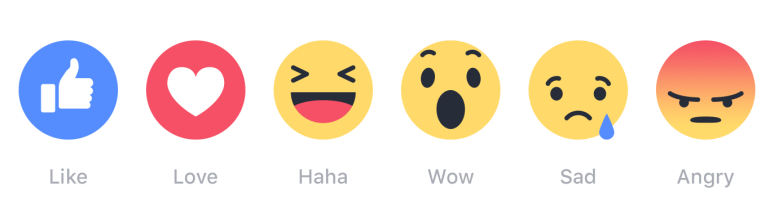
\includegraphics[scale=.2]{reactions-image-en_us.png}
%  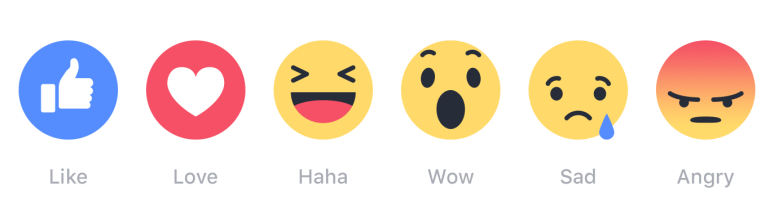
\includegraphics[scale=.25]{reactions-image-en_us.png}
  \caption{Facebook reactions}
  \label{fig:facebook_reactions}
\end{wrapfigure}
In February 2016, after a short trial, Facebook made a more explicit \textit{reaction} feature available world-wide. Rather than allowing for the underspecified ``like'' as the only wordless response to a post, a set of more specific reactions was introduced, as shown in Figure \ref{fig:facebook_reactions}: \texttt{Like, Love, Haha, Wow, Sad and Angry}. We use such reactions as proxies for emotion labels associated to posts.

We collected Facebook posts and their corresponding reactions from public pages using the Facebook API, which we accessed via the Facebook-sdk python library\footnote{https://pypi.python.org/pypi/facebook-sdk}. We chose different pages (and therefore domains and stances), aiming at a balanced and varied dataset, but we did so mainly based on intuition (see Section~\ref{sec:model}) and with an eye to the nature of the datasets available for evaluation (see Section~\ref{sec:evaluation}). The choice of which pages to select posts from is far from trivial, and this is actually an interesting aspect of our approach, as by using different Facebook pages one can intrinsically tackle the domain-adaptation problem (See Section~\ref{sec:conclusions} for further discussion on this). The final collection of Facebook pages is as follows: 
\texttt{FoxNews}, 
\texttt{CNN}, 
\texttt{ESPN}, 
\texttt{New York Times}, 
\texttt{Time magazine},
\texttt{Huffington Post Weird News}, 
\texttt{The Guardian}, 
\texttt{Cartoon Network}, 
\texttt{Cooking Light}, 
\texttt{Home Cooking Adventure}, 
\texttt{Justin Bieber}, 
\texttt{Nickelodeon}, 
\texttt{Spongebob}, 
\texttt{Disney}
.
%can be seen in Figure~\ref{fig:distribution_facebook}.
%These combinations of posts and the corresponding reactions can be used for training a emotion classifier by for example using the emotion most used as label. 


\begin{wrapfigure}{r}{8cm}
\vspace*{-.8cm}
\begin{Verbatim}[fontsize=\scriptsize]
[
 {
  "created_time": "2016-06-19T01:40:00+0000",
  "message": "Walt Disney World representatives said 
  they plan to put up fencing and signs at all resorts 
  and waterways.",
  "reactions": [5073, 4483, 60, 22, 54, 284, 170, 0]
 }
],
[
 {
  "created_time": "2016-06-19T01:00:00+0000",
  "message": "Charlene and Joseph Handrik face more
  than 550 counts of animal cruelty.",
  "reactions": [2256, 1011, 16, 6, 123, 409, 691, 0]
 }
],
\end{Verbatim}
\vspace*{-.8cm}
\caption{Sample of resulting JSON file\label{fig:json}. The order of values/reactions is \texttt{total, like, love, haha, wow, sad, angry, thankful}.}
\end{wrapfigure}


For each selected page, we downloaded the latest 1000 posts, or the maximum available if there are fewer, from February 2016,
%, which is when the reaction feature was introduced. 
retrieving the counts of reactions for each post. The output is a JSON file containing a list of dictionaries with a timestamp, the post and a reaction vector with frequency values. The emotion vectors must then be turned into an emotion label.\footnote{Note that \texttt{thankful} was only available during specific time spans related to certain events, as Mother's Day in May 2016.}

In the context of this experiment, we made the simple decision of associating to each post the emotion with the highest count, ignoring \texttt{like} as it is the default and most generic reaction people tend to use. Therefore, for example, to the first post in Figure~\ref{fig:json}, 
  we would associate the label \texttt{sad}, as it has the highest score (284) among the meaningful emotions we consider, though it also has non-zero scores for other emotions. At this stage, we didn't perform any other entropy-based selection of posts, to be investigated in future work.

%as shown in Figure~\ref{fig:json} (the order of reactions is \texttt{total, like, love, haha, wow, sad, angry, thankful}).



%\begin{figure}
%  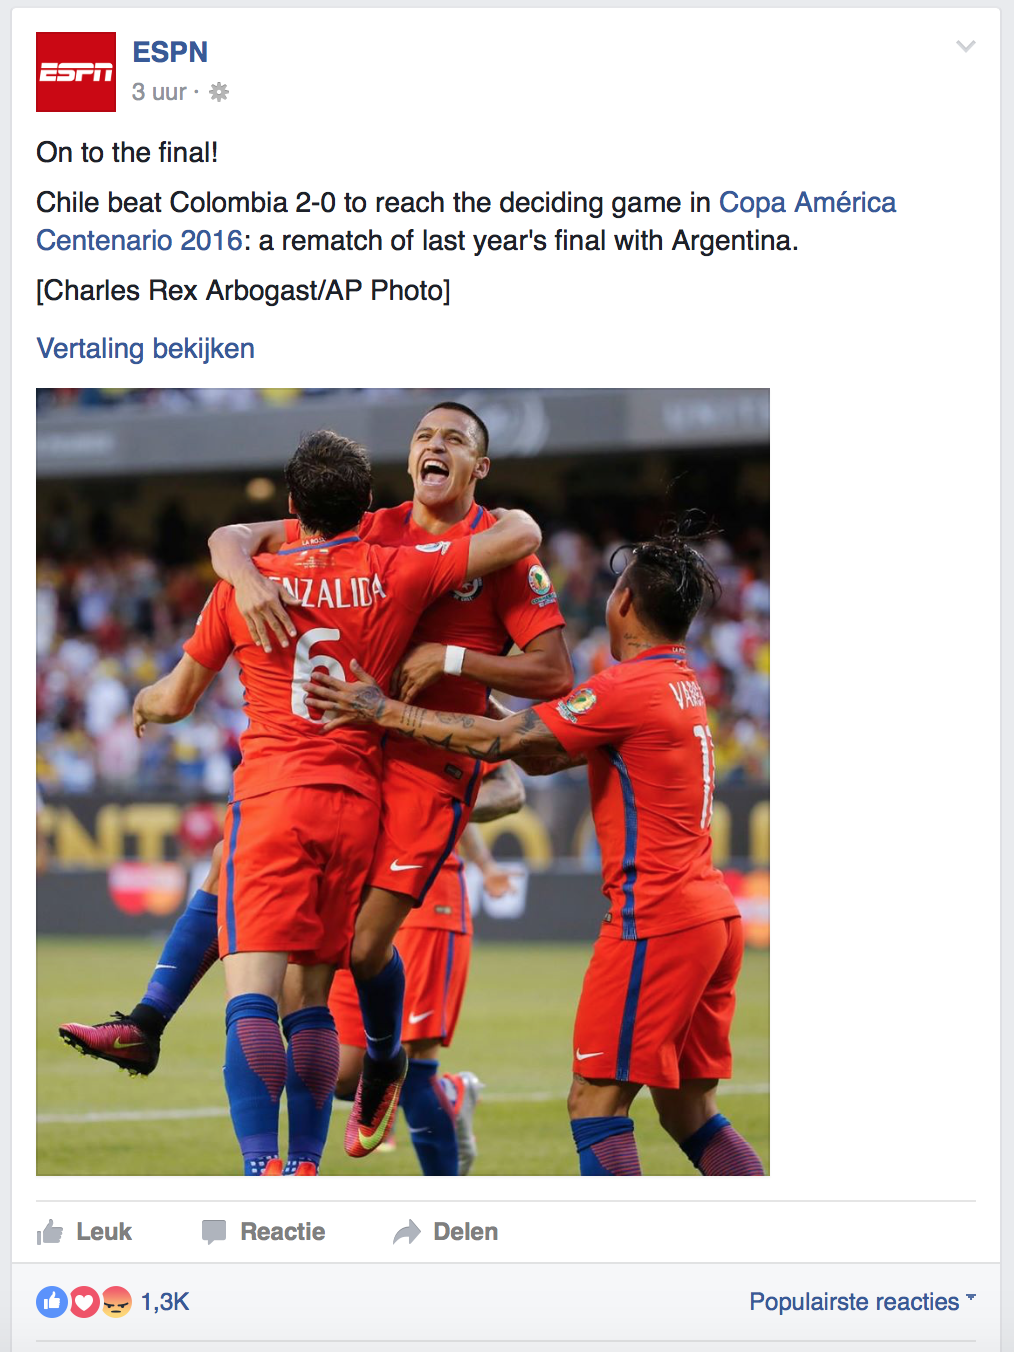
\includegraphics[width=\linewidth]{facebook_post_football.png}
%  \caption{Post on Facebook}
%  \label{fig:facebook_reactions_post_football}
%\end{figure}

%\subsection{Using the API}
%The Facebook API enables developers to interact with data available on Facebook, depending on the permissions you have. Using the API requires a developers account that easily can be created on \verb+http://developers.facebook.com+. For getting my training data I created a script (get\_facebook\_reactions.py) that can be found in the GitHub repo. First it downloads the last 1000 posts if available since February 2016, the period Facebook started with the reactions. For my scripts I used the excellent Python Facebook library written by Martey Dodoo \footnote{https://pypi.python.org/pypi/facebook-sdk}. 

%\begin{lstlisting}[language=Python, caption=Script that retrieves the posts from a Facebook page]
%#download all posts from the CNN page
%cnn_posts = get_all(graph.get_object(id="cnn/feed"))
%for post in cnn_posts:
%        
%  try:
%    # Perform some action on each post in the collection
%    #  we receive from Facebook.
%    cnn_posts.extend(items['data'])
%    # Attempt to make a request to the next page of 
%    # data, if it exists.
%    items = requests.get(items['paging']['next']).json()
%  except KeyError:
%    # When there are no more pages break from the
%    # loop and end the script.
%    print("....Finished getting data")
%    break
%\end{lstlisting}

%The snippet above retrieves the first 20 posts using the code on line 2. Each request to the API is limited to 20 items being returned but contains the url for the next 20 items. I use this url in a for loop, where I continue querying the webservice until there are no more pages available, resulting in a list of posts. \\\\



%\begin{lstlisting}[language=Python, caption=Retrieving emotion vector using Facebook API]
%possible_reactions = ['NONE', 
%                      'LIKE', 
%                      'LOVE', 
%                      'HAHA', 
%                      'WOW', 
%                      'SAD', 
%                      'ANGRY', 
%                      'THANKFUL']
%for i, post in enumerate(cnn_posts):      
%        if 'message' in post: #filter out events
%            reaction_vector = []
%            for reaction in possible_reactions:
%                rs = graph.get_object(id="{}?fields=reactions.type({})
%.summary(true)" .format(post['id'], reaction))
%                                     
%                reaction_vector.append(rs['reactions']['summary']['total_count'])
%  
%            result.append([{'created_time': post['created_time'], 
%                            'message': post['message'], 
%                            'reactions': reaction_vector}])
%\end{lstlisting}
%The final result list contains a list of dictionaries with a timestamp, message and a reaction vector. This is written to a JSON file as can be seen in the code example below.
%

%\subsection{Choosing Facebook pages}

%Choosing what pages to select is not trivial. 
%For my experiment I collected the posts from several Facebook pages from different domains to get a good balanced data set. I chose the pages primarily based on intuition. For the experiment I want to select the pages that are most similar to the target domain. The results per Facebook page and which pages I ended up using can be found in the Experiment section. 





\section{Emotion datasets}
\label{sec:emoData}

Three datasets annotated with emotions are commonly used for the development and evaluation of emotion detection systems. In order to compare our performance to state-of-the-art results, we have used them as well. In addition to a description of each dataset, we provide an overview of the emotions used, their distribution, and how we mapped them to those we obtained from Facebook posts in Section~\ref{sec:overview}.

\subsection{Affective Text dataset}
\label{sec:data:affect}
Task~14 at SemEval~2007  \cite{strapparava2007semeval} was concerned with the classification of emotions and valence in news headlines. The headlines where collected from several news websites including Google news,  The New York Times, BBC News and CNN. The used emotion labels were \texttt{Anger, Disgust, Fear, Joy, Sadness, Surprise}), in line with the basic emotions of Ekman's standard model \cite{ekman1992argument}. Valence was to be determined as positive or negative. Classification of emotion and valence were treated as separate tasks. 
Emotion labels were not considered as mututally exclusive, and each emotion was assigned a score from 0~to~100. Training/developing data amounted to 250 annotated headlines, while systems were evaluated on another 1000. Evaluation was done using two different methods: a fine-grained evaluation using Pearson's \textit{r}  to measure the correlation between the system scores and the gold standard. With a coarse-grained method, each emotion score was converted to a binary label, and precision, recall, and f-score were used for evaluation. As it is done in most works that use this dataset \cite{kim2010evaluation,chaffar2011using,calvo2013emotions}, we treat this as a classification problem (coarse-grained).  This dataset has been extensively used for the evaluation of various unsupervised techniques \cite{strapparava2008learning}, but also for testing different supervised learning techniques and feature portability \cite{mohammad:2012:NAACL-HLT}.

%
%
%In most researches, the vector of emotion was converted to a categorical label, in all researches the emotion with the highest value was used (\cite{chaffar2011using}, \cite{calvo2013emotions} and \cite{kim2010evaluation}).
%In the paper by \cite{kim2010evaluation} they evaluated several unsupervised techniques using, among others, this data-set (see Section~\ref{sec:evaluation} for results). The results, reported in precision, recall and f-score can be found in section 5. also used this data-set to evaluate five different unsupervised techniques . The results are also reported using precision, recall and f-score for each emotion category. \cite{mohammad:2012:NAACL-HLT}.

%
%\paragraph{Technical description}
%The data-set consists of four files. For the development and test-set both two XML files are used. One XML file contains the headlines with an ID, the other XML file contains the emotion vector (score for each emotion).
%\begin{figure}[htb]
%  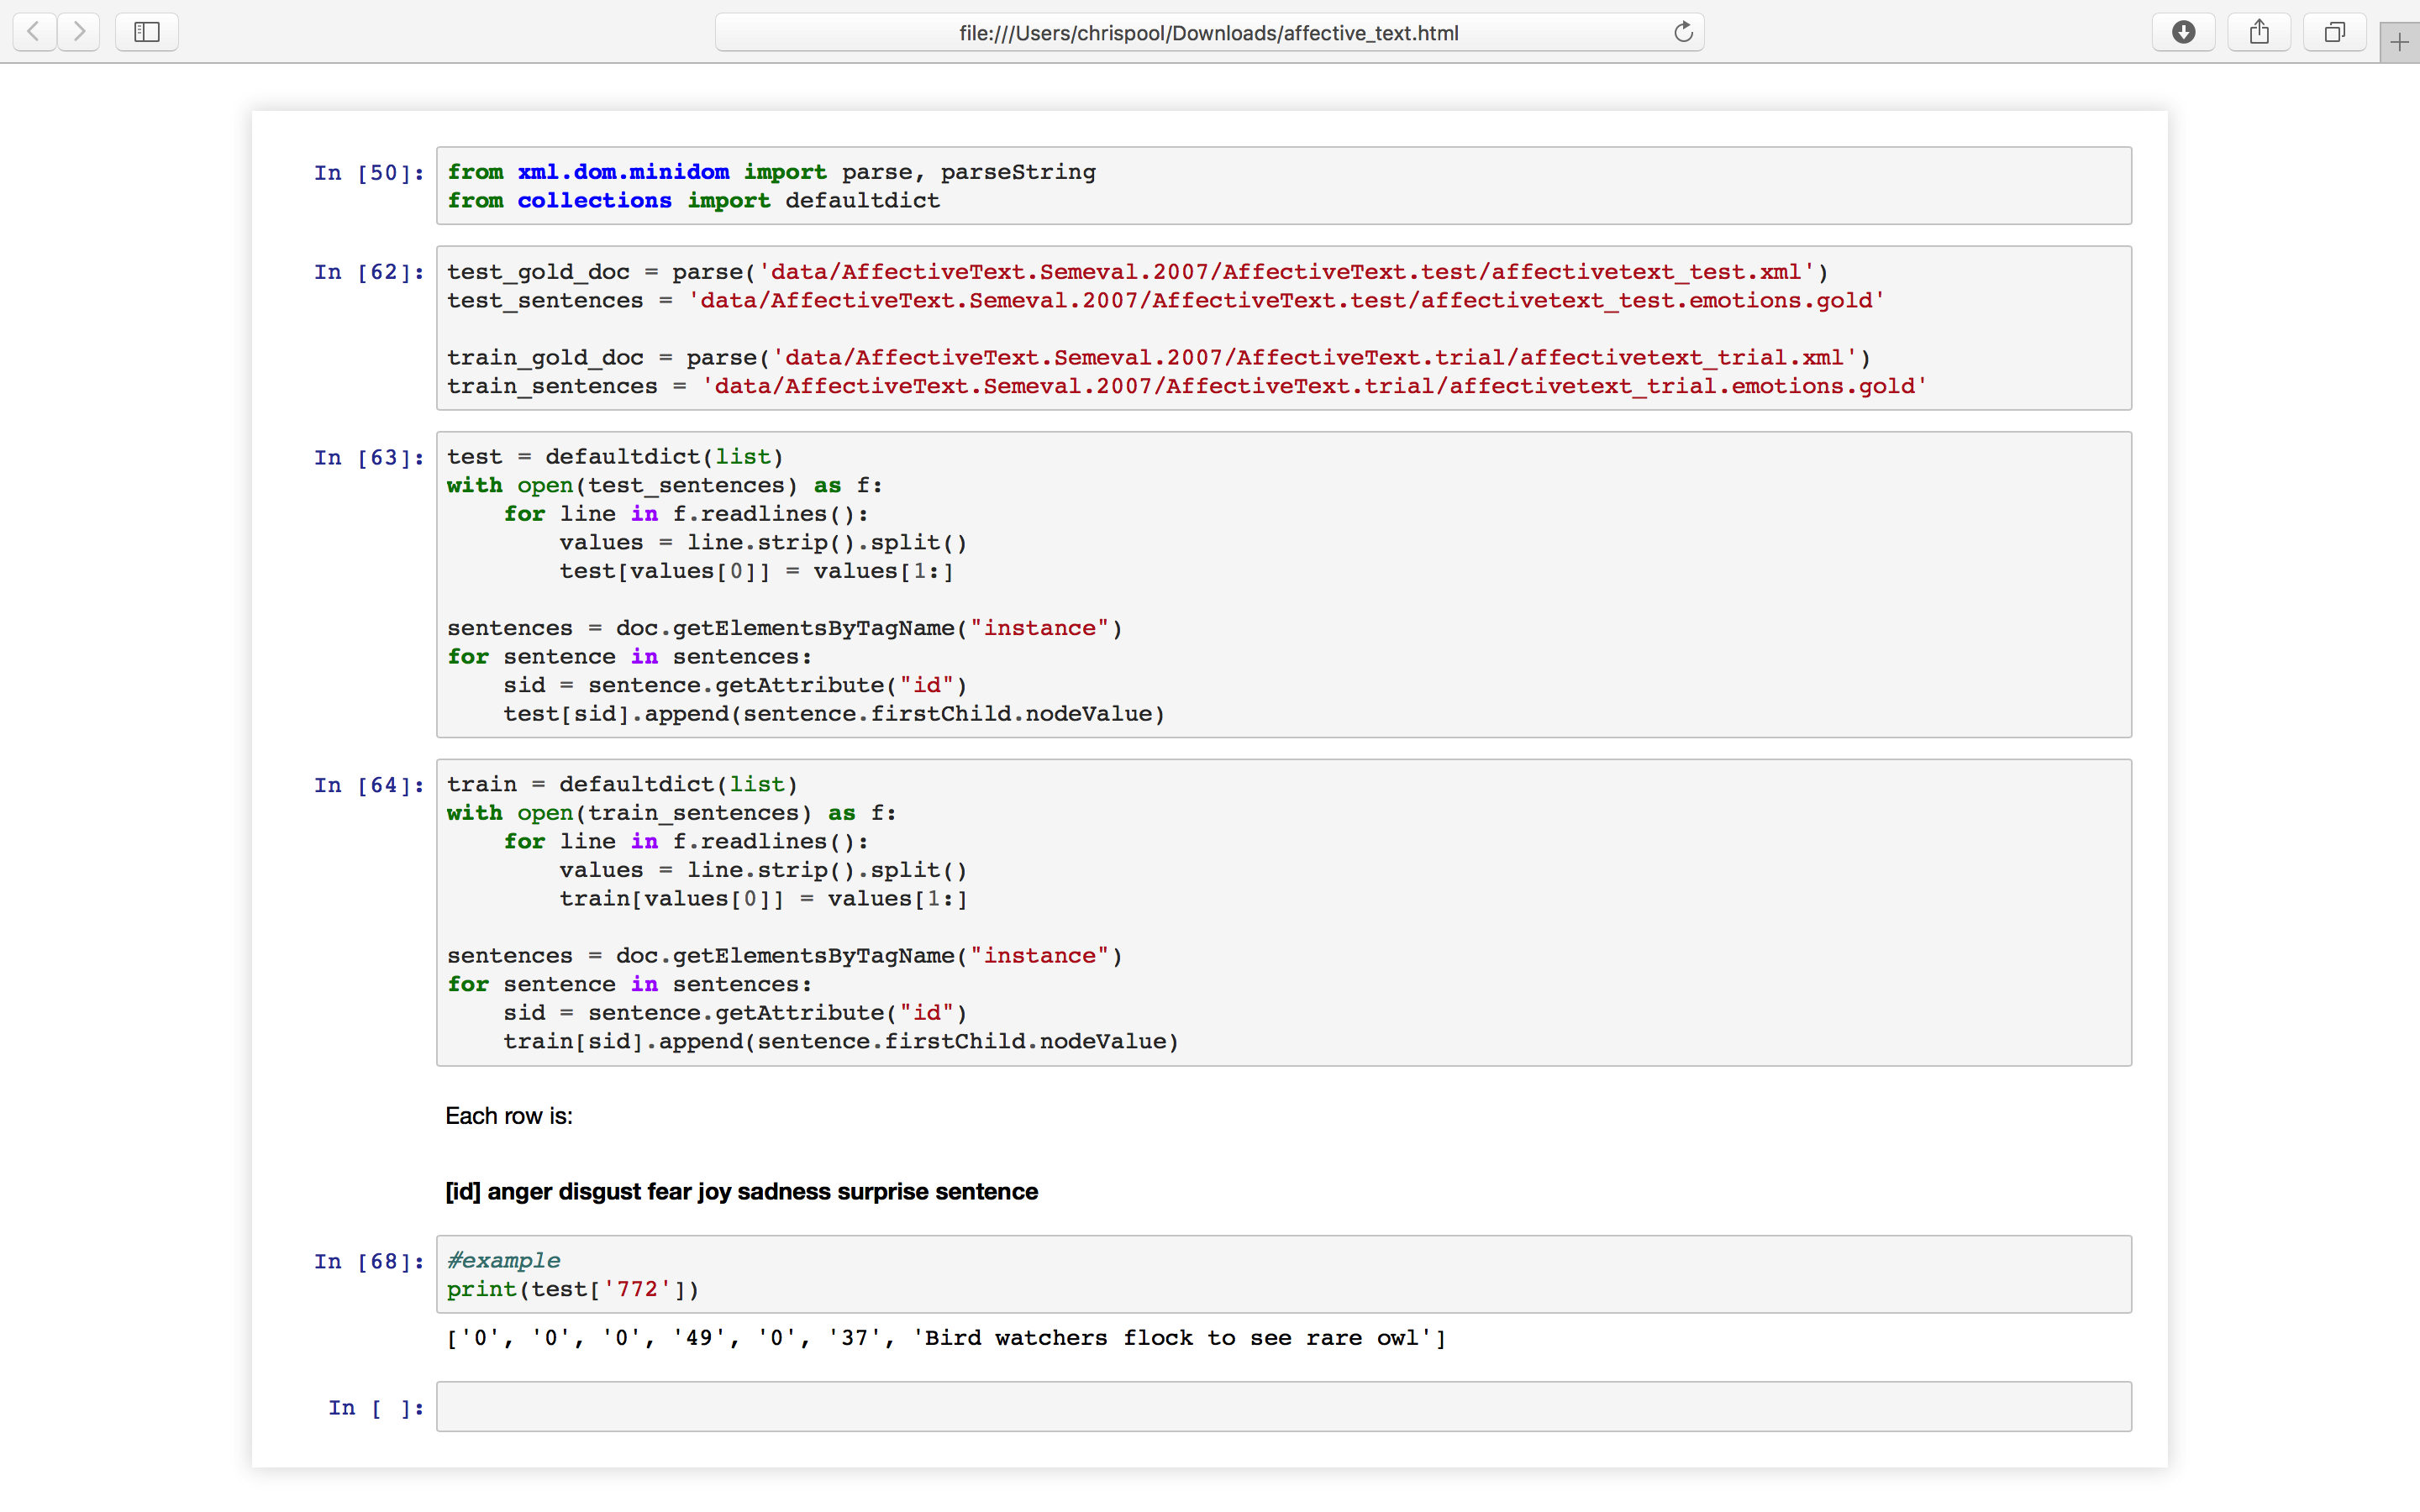
\includegraphics[width=\linewidth]{dataset_affective.png}
%  \caption{Parsing the data-set using Jupyter Notebook (affective\_text.py)}
%  \label{fig:dataset_affective}
%\end{figure}
%Figure \ref{fig:dataset_affective} is an example how to parse the data. The emotion vector indicates a strong Joy and Surprise emotion for the sentence 


%Example sentence from the dataset: \texttt{`Bird watchers flock to see rare owl`}, emotions: Joy and Surprise \note{check commented out figure}.


\subsection{Fairy Tales dataset}
This is a dataset collected by \newcite{alm2008affect}, where about 1,000 sentences from fairy tales (by B. Potter, H.C. Andersen and Grimm) were annotated with the same six emotions of the Affective Text dataset, though with different names: \texttt{Angry}, \texttt{Disgusted}, \texttt{Fearful}, \texttt{Happy}, \texttt{Sad}, and \texttt{Surprised}. In most works that use this dataset \cite{kim2010evaluation,chaffar2011using,calvo2013emotions}, only sentences where all annotators agreed are used, and the labels \texttt{angry} and \texttt{disgusted} are merged. We adopt the same choices. 
%The Affective Labels are in most researches: Angry-Disgusted, Fearful, Happy, Sad, and Surprised. I followed this mapping.

% Description of the dataset
%The dataset contains four folders containing the raw data where for each sentence there are four annotations. A data-set that only contains the sentences with a high agreement are stored in a different folder and is used for most researches. The definition of high agreement is in this case where all the four labels are the same.

%In our experiments this dataset is only used for the final testing.

 


%\begin{figure}[htb]
%  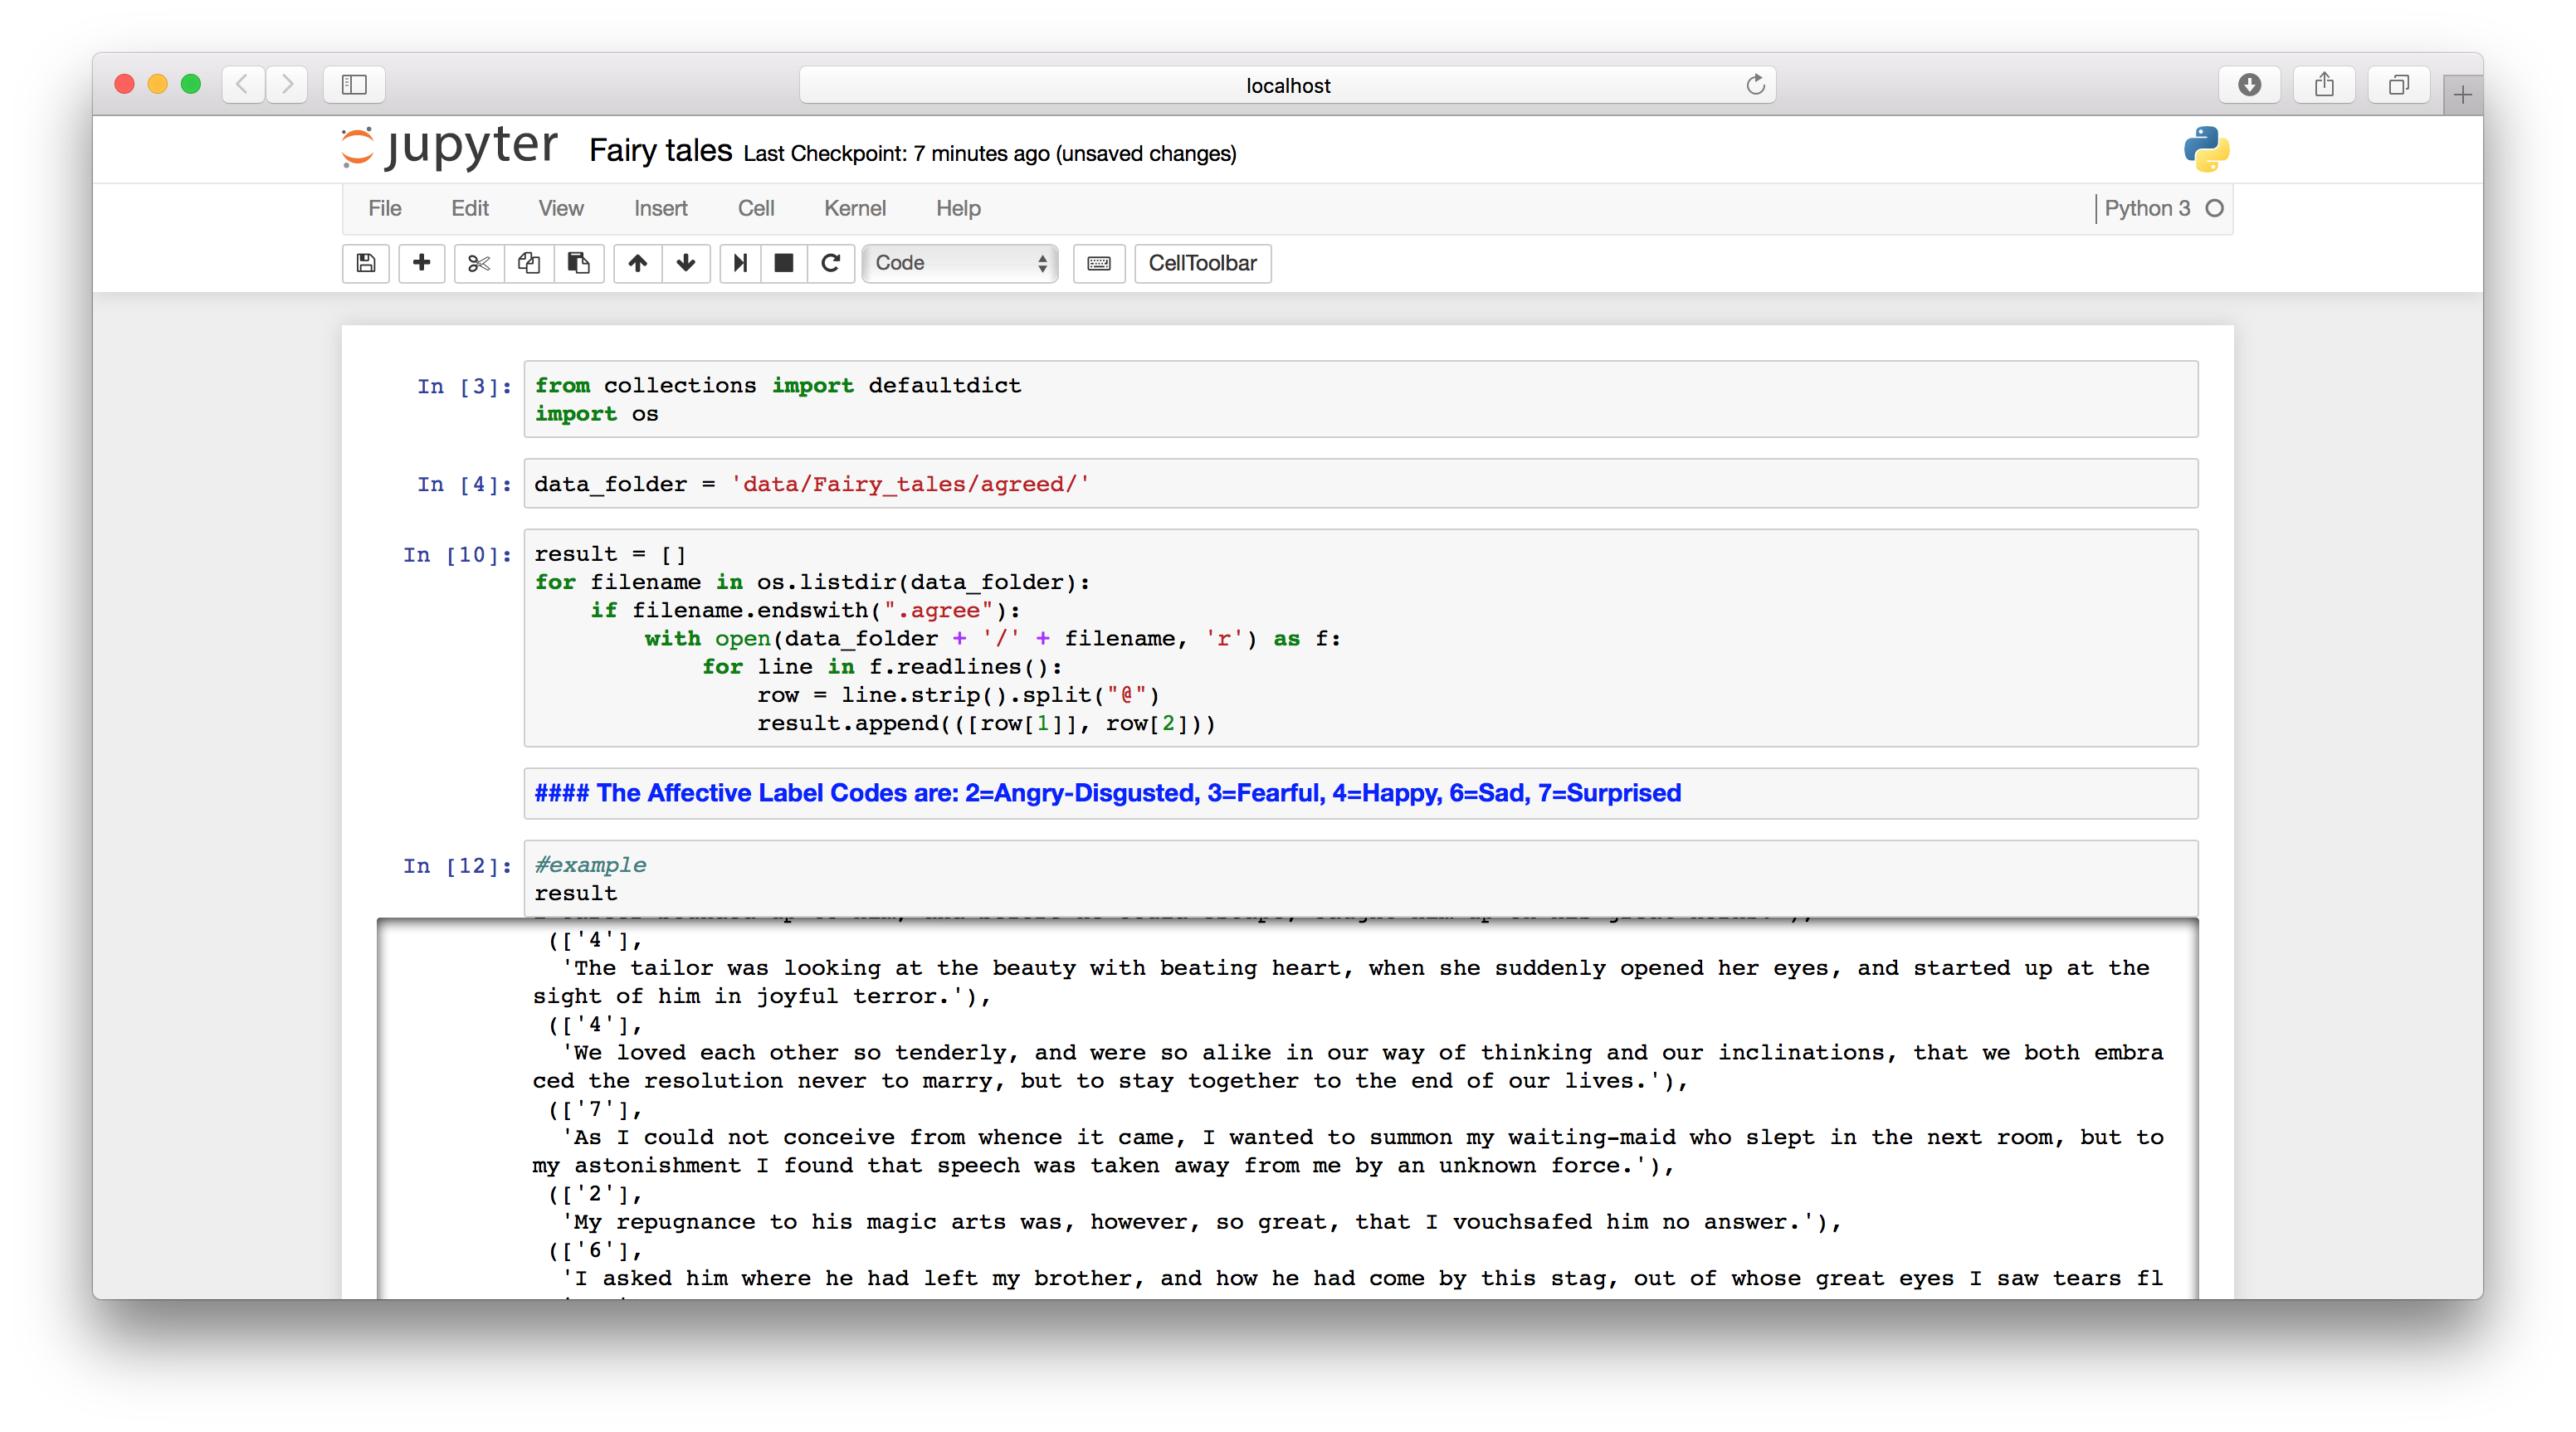
\includegraphics[width=\linewidth]{dataset_fairy-tales.png}
%  \caption{Parsing the dataset using Jupyter Notebook (fairy-tales.py}
%  \label{fig:dataset_fairy-tales}
%\end{figure}

%Figure \ref{fig:dataset_fairy-tales} is an example how to parse the data. Each item in the list is a tuple of the emotion and the sentence, an example can be found below.

%Example sentence from dataset: ``We loved each other so tenderly, and were so alike 
%in our way of thinking and our inclinations, that we both 
%embraced the resolution never to marry, but to stay together 
%to the end of our lives.'' with joy emotion.


%In the documentation can be found that the \texttt{4} indicates a Joy full emotion.


\subsection{ISEAR}
\label{sec:data:isear}
The ISEAR (International Survey on Emotion Antecedents and Reactions) is a dataset created in the context of a psychology project of the 1990s, by collecting questionnaires answered by people with different cultural backgrounds.   Student respondents, both psychologists and non-psychologists, were asked to report situations in which they had experienced all of 7 major emotions (\texttt{joy, fear, anger, sadness, disgust, shame} and \texttt {guilt}). In each case, the questions covered the way they had appraised the situation and how they reacted. The final dataset contains reports on seven emotions, by approximately 3000 respondents from all over the world.
%The data is stored in a Microsoft Access database where each row contains, among other information, the emotion and the sentence. 
In total there are 7665 sentences labelled with an emotion, making this the largest testset out of the three we use. 

%In our experiments this dataset is only used for the final testing.

%Questions were about personal experiences which could be labelled with one of 
%that contains 7,665 sentences. The data-set is created by using questionnaires from participants with different cultural backgrounds. The questionnaires contained questions about experiences and reactions for seven emotions including: 
%\texttt{anger, disgust, fear, joy, sadness, shame and guilt}. 



% Overview in which papers this data set was used





\subsection{Overview of datasets and emotions}
\label{sec:overview}

We summarise datasets and distribution from two viewpoints. First, because there are different sets of emotions labels in the datasets and Facebook data, we need to provide a mapping and derive a subset of emotions that we are going to use for the experiments. This is shown in Table~\ref{overview_data-sets}, where in the ``Mapped'' column we report the final emotions we use in this paper: \texttt{anger, joy, sadness, surprise}. 
\begin{wraptable}{r}{10cm}
\vspace*{-.5cm}
\begin{footnotesize}
\caption{Mapping emotions\label{overview_data-sets}}
\centering
\begin{tabular}{|l|l|l|l|l|}
\hline
\textbf{Affect. T.} & \textbf{Fairy tales} & \textbf{ISEAR} & \textbf{Facebook} & \textbf{Mapped} \\ \hline
Anger            & Angry-Disgusted      & Anger               & Angry   & ANGER          \\ \hline
Disgust          & Angry-Disgusted      & Disgust               &    &  ANGER              \\ \hline
Fear             & Fearful              & Fear               &      &              \\ \hline
Joy              & Happy                & Joy                & Haha, Love & JOY\\ \hline
Sadness          & Sad                  & Sadness               & Sad     & SADNESS          \\ \hline
Surprise         & Suprised             &                & Wow          & SURPRISE     \\ 
\hline
                 &                      & Shame               &       &         \\ \hline
                 &                      & Guilt               &       &         \\                  
\hline
\end{tabular}
\end{footnotesize}
\end{wraptable}
Second, the distribution of the emotions for each dataset is different, as can be seen in Figure~\ref{fig:distribution_data-sets}. 

In Figure~\ref{fig:distribution_facebook} we also provide the distribution of the emotions \texttt{anger, joy, sadness, surprise} per Facebook page, in terms of number of posts (recall that we assign to a post the label corresponding to the majority emotion associated to it, see Section~\ref{sec:FBData}). We can observe that for example pages about news  tend to have more sadness and anger posts, while pages about cooking and tv-shows have a high percentage of joy posts. We will use this information to find the best set of pages for a given target domain (see Section~\ref{sec:evaluation}).






\begin{figure}[hbt]
\begin{minipage}{.48\textwidth}
  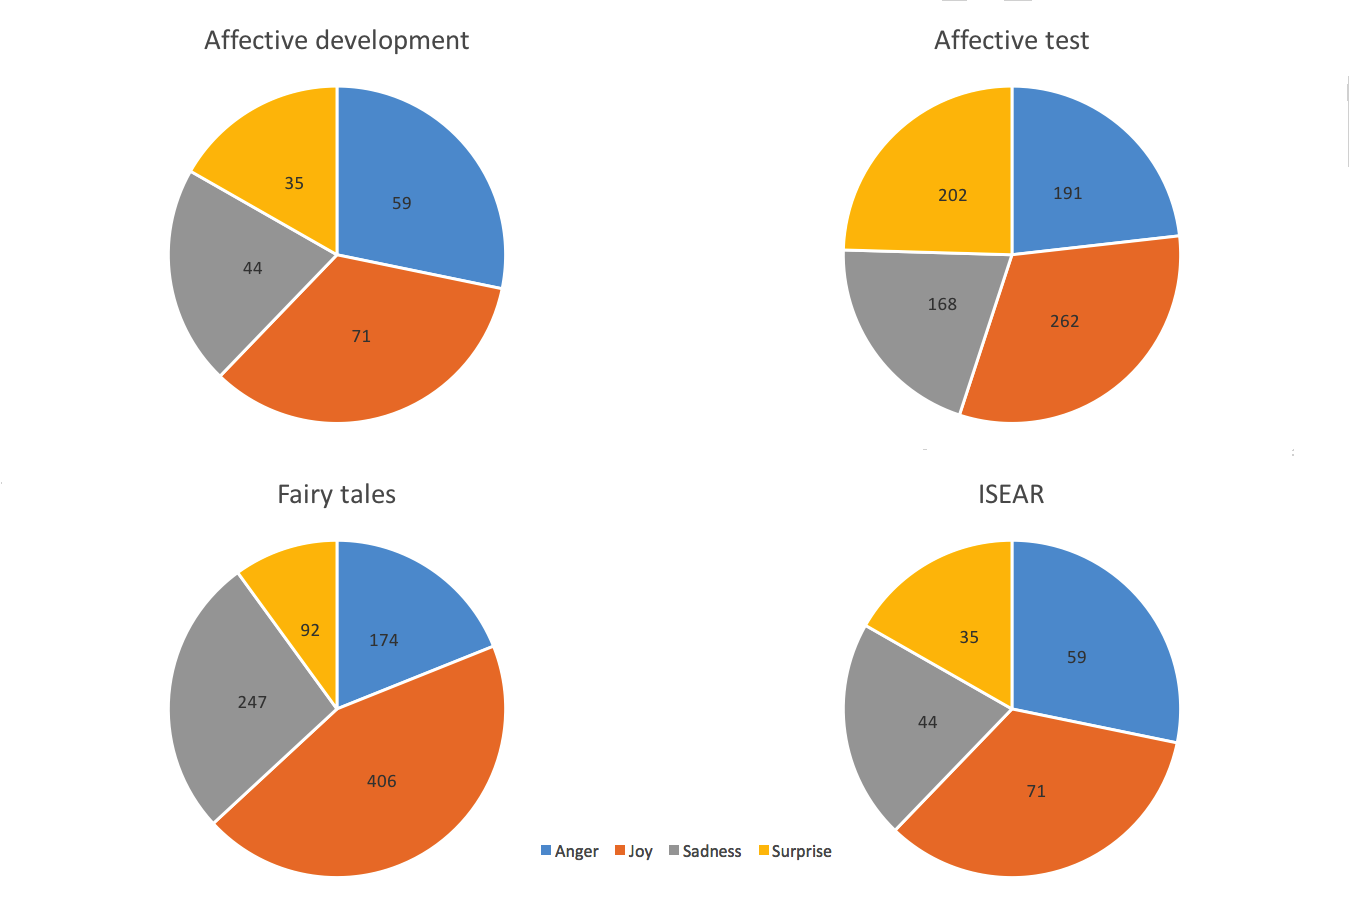
\includegraphics[scale=.145]{distribution_data.png}
  \caption{Distribution of emotions in the datasets  \label{fig:distribution_data-sets}}
\end{minipage}
\begin{minipage}{.48\textwidth}
%\begin{sidewaysfigure}
    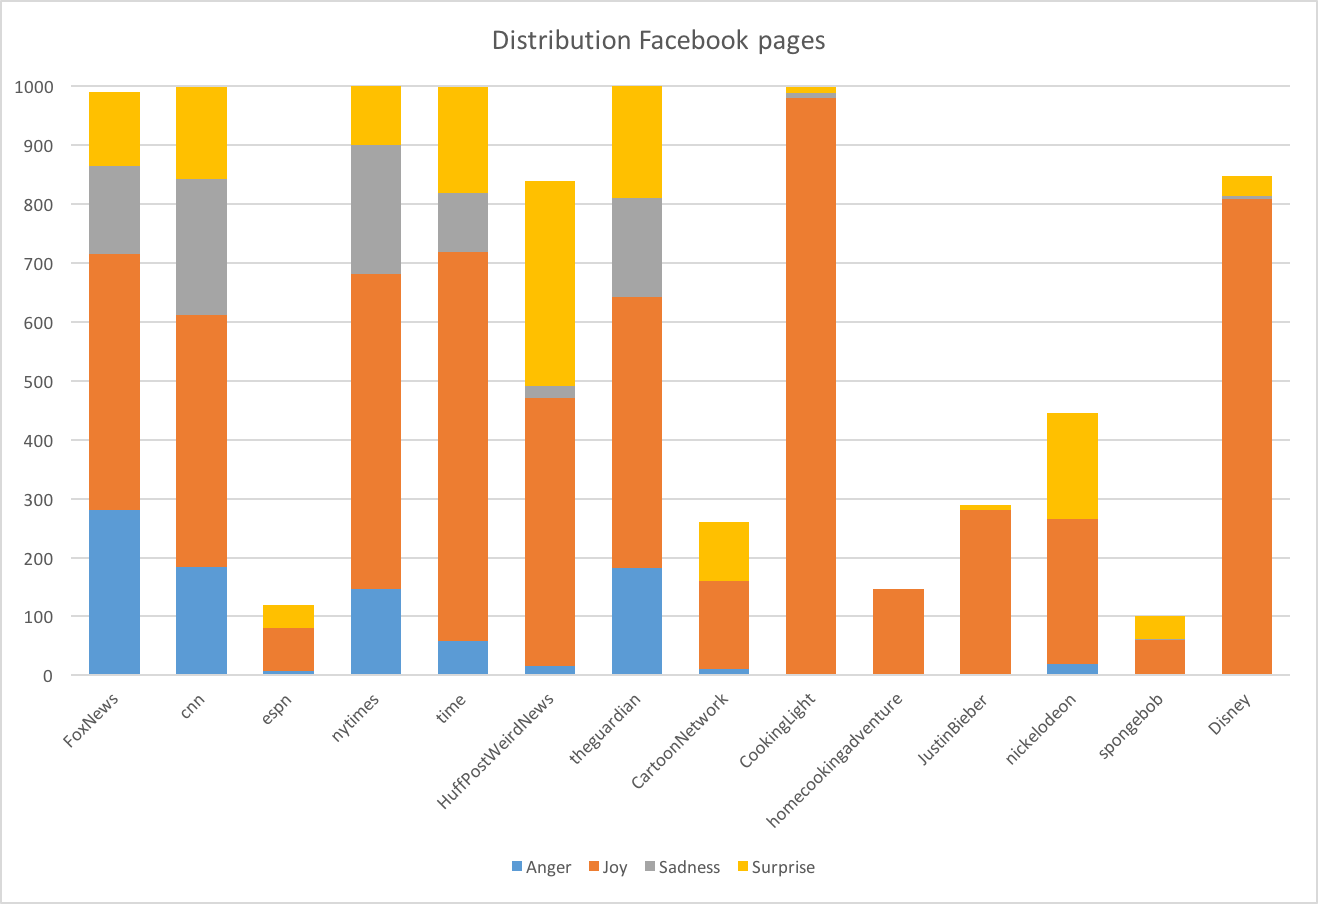
\includegraphics[scale=.3,keepaspectratio]{distribution_facebook.png}  
\caption{Distribution of posts per page\label{fig:distribution_facebook}}
%\end{sidewaysfigure}
\end{minipage}
\end{figure}


%In table \ref{overview_data-sets} an overview can be found of emotions used in the datasets described in the previous sections. For developing my system the intersection of emotions are used and are mentioned in the \texttt{Mapped} column.


%\begin{tabular}{lrrrrrl}
%dataset & size & anger & joy & sadness & surprise & function\\
%\hline
%SemEval\_dev & & & & & dev\\
%Semeval\_test & & & & & test \\
%FairyTales    & & & & & test \\
%ISEAR  && & & & test\\
%\hline
%\end{tabular}




\section{Model}
\label{sec:model}

% mention SVM

There are two main decisions to be taken in developing our model: (i) which Facebook pages to select as training data, and (ii) which features to use to train the model, which we discuss below. Specifically, we first set on a subset of pages and then experiment with features. Further exploration of the interaction between choice of pages and choice of features is left to future work, and partly discussed in Section~\ref{sec:conclusions}. For development, we use a small portion of the Affective data set described in Section~\ref{sec:data:affect}, that is the portion that had been released as development set for SemEval's 2007 Task~14 \cite{strapparava2007semeval}, which contains 250 annotated sentences. All results reported in this section are on this dataset.
  The test set of Task~14 as well as the other two datasets described in Section~\ref{sec:emoData} will be used to evaluate the final models.


%  All results reported in this Section are obtained on the development portion of the Affective dataset (Section~\ref{sec:data:affect}).

%By parsing the resulting JSON files that are described in Section~\ref{sec:FBData}, for each retrieved post we select the emotion with the highest count as a training label for that post. 


\subsection{Selecting Facebook pages}
\label{sec:selecting}

Although page selection is a crucial ingredient of this approach, for the experiments described here we took a rather simple approach, by first selecting the pages that would provide training data based on intuition and availability, then choosing different combinations according to results of a basic model run on development data, and eventually testing feature combinations, still on the development set.

%We explored potential correlations between the number of posts per emotion and the performance of the model for that emotion. 
For the sake of simplicity and transparency, we first trained an SVM with a simple bag-of-words model and default parameters as per the Scikit-learn implementation \cite{scikit-learn} on different combinations of pages. Based on results of the attempted combinations as well as on the distribution of emotions in the development dataset (Figure~\ref{fig:distribution_data-sets}), we selected a \textit{best model} (\textbf{B-M}), namely the combined set of \texttt{Time, The Guardian} and \texttt{Disney}, which yields the highest results on development data. \texttt{Time} and \texttt{The Guardian} perform well on most emotions but \texttt{Disney} helps to boost the performance for the \texttt{Joy} class.


\subsection{Features}
In selecting appropriate features, we mainly relied on previous work and intuition. We experimented with different combinations, and all tests where done on the development portion of the Affective Text dataset, using the pages for the best model (B-M) described above as training data. %The contribution of the features to our models performance can be found 
Results are in Table~\ref{test_results_svm}.
Future work will further explore the simultaneous selection of features and page combinations.


%Because the training data is from a different domain then the target domain the challenge is to create general models that are not domain specific. 
%The evaluation of used features is done on the Affective text data-set. The final evaluation is done on other data from other domains. 


\paragraph{Standard textual features} We use a set of basic text-based features to capture the emotion class. These include a tf-idf bag-of-words feature, word (2-3) and character (2-5) ngrams, and features related to the presence of negation words, and to the usage of punctuation.

%\paragraph{Negation and Punctuation}
%Negation is the grammatical operation whereby a proposition is replaced by one that states the opposite. An affirmative form expresses the validity or truth of a basic assertion. A negative form expresses the falsity of a basic assertion. In the English language, sentences may be negated with the adverbs \textit{not} and \textit{never}, the determiner \textit{no}, and the indefinite pronouns \textit{no one}, \textit{nobody}, and \textit{none} as well as other negative words.

%\paragraph{Bag of words}
%This basic features uses words as feature. I used the TF-idf, which is a measure to assign a weight to important words. Words that appear in each document are less relevant since it doesn\'t help in classification.
%
%\paragraph{N-grams}
%N-gram-based features have proven to be a good performing feature in various researches about emotion detection. At the token level, features with uni-grams, bi-grams and tri-grams were implemented. The character-level features consisted of n-grams of 2 to 5 characters. 

\paragraph{Affect Lexicons} this feature is used in all unsupervised models as a source of information, and we mainly use it to assess its contribution, but eventually don't include it in our final model. 
%We use the NRC10 lexicon because it was shown to perform best in \cite{mohammad:2012:NAACL-HLT}.

%\cite{Mohammad:13}
% \note{which is also used in other emotion classification experiments.}
%\newcite{mohammad:2012:NAACL-HLT} explores the performance of the different lexicons: NRC10  and WordNet Affect\cite{strapparava2004wordnet}. 
We used the NRC10 lexicon as lexicon because it performed best in the experiments by \cite{mohammad:2012:NAACL-HLT}, which is built around the emotions \texttt{anger}, \texttt{anticipation}, \texttt{disgust}, \texttt{fear}, \texttt{joy}, \texttt{sadness}, and \texttt{surprise}, and the valence values \texttt{positive} and \texttt{negative}. For each word in the lexicon, a boolean value indicating presence or absence is associated to each emotion. For a whole sentence, a global score per emotion can be obtained by summing the vectors for all content words of that sentence included in the lexicon, and used as feature.
%The score for a sentence can be
%'negative', 'positive', 'sadness', 'surprise', 'trust'For each word in the lexicon there is a Boolean value whether it contains that emotion or not. For example the word \texttt{FUN}:
%\begin{lstlisting}[language=python]
%fields = ['anger', 'anticipation', 'disgust', 'fear', 'joy',
%'negative', 'positive', 'sadness', 'surprise', 'trust']
%fun  = [0,1,0,0,1,0,1,0,0,0]
%
%[field for field, fun in zip(fields, fun) if fun == 1]
%--> 'anticipation', 'joy', 'positive'
%\end{lstlisting}


% as can be seen in table \ref{feature_lexicon}.
%
%\begin{table}[hbt]
%\centering
%
%
%\begin{tabular}{ll}
%
%victims                            & {[}1, 0, 0, 1, 0, 1, 0, 1, 0, 0{]}                               \\
%terror                             & {[}0, 0, 0, 1, 0, 1, 0, 0, 0, 0{]}                               \\
%attack                             & {[}1, 0, 0, 1, 0, 1, 0, 0, 0, 0{]}                               \\
%remembered                         & {[}0, 0, 0, 0, 0, 0, 0, 0, 0, 0{]}                               \\
%tribute                            & {[}0, 0, 0, 0, 0, 0, 1, 0, 0, 0{]}                               \\
%National                           & {[}0, 0, 0, 0, 0, 0, 0, 0, 0, 0{]}                               \\
%Memorial                           & {[}0, 0, 0, 0, 0, 0, 0, 0, 0, 0{]}                               \\ \hline
%\textbf{SUM} & {[}2, 0, 0, 3, 0, 3, 1, 1, 0, 0{]} \\ 
%\end{tabular}
%\caption{Score for \texttt{'victims of the terror attack in Orlando are remembered in a tribute at the National September 11 Memorial \& Museum.'}}
%\label{feature_lexicon}
%\end{table}
%

\paragraph{Word Embeddings}
As additional feature, we also included Word Embeddings, namely distributed representation of words in a vector space which have been exceptionally successful in boosting performance in a plethora of NLP tasks.% that must rely on small amounts of labelled data. 
We use three different embeddings: 

\begin{itemize} 

\item \textit{Google embeddings}: pre-trained embeddings trained on Google~News and obtained with the skip-gram architecture described in  \cite{mikolov2013distributed}. This model contains 300-dimensional vectors for 3 million words and phrases.

\item \textit{Facebook embeddings}: embeddings that we trained on our scraped Facebook pages for a total of 20,000 sentences. Using the \texttt{gensim} library \cite{gensim}, we trained the embeddings with the following parameters: window size of 5, learning rate of 0.01 and dimensionality of 100. We filtered out words with frequency lower than 2 occurrences.

\item \textit{Retrofitted embeddings}: 
%generally learned embeddings that are refined using information about relations between words derived from external resources, such as semantic lexica and ontologies. This information is fed back, i.e. \textit{retrofitted}, to the embeddings, so that words that are linked by relations such as hyponymy for example, can get closer in space 
Retrofitting \cite{retrofitting} has been shown as a simple but efficient way of informing trained embeddings with additional information rather than including it directly at the training stage, as it's done for example to create sense-aware \cite{iacobacci2015sensembed} or sentiment-aware \cite{tang:14} embeddings.\footnote{Training emotion-aware embeddings is a strategy that we plan to explore in future work.} In this work, we retrofit general embeddings to include information about emotions, so that emotion-similar words can get closer in space. Both the Google as well as our Facebook embeddings were retrofitted with lexical information obtained from the NRC Lexicon. Note that differently from the previous two types of embeddings, the retrofitted ones do rely on handcrafted information in the form of a lexical resource.


%\note{Facebook-built (small but appropriate), general google embeddings, and retrofitted embeddings (which however rely again on hand-crafted info). Remember to cite.}


\end{itemize}

\subsection{Results on development set}

We report precision, recall, and f-score on the development set. The average f-score is reported as \textit{micro-average}, to better account for the skewed distribution of the classes as well as in accordance to what is usually reported for this task \cite{mohammad2015using}.

\begin{table*}[!htbp]
\caption{Results on the development set\label{test_results_svm}}
\centering
\begin{tabular}{|l|c|c|c|c|c|}
\hline
    & \texttt{anger} & \texttt{joy} & \texttt{sadness} & \texttt{surprise} &  \\ 
    \hline
          Feature         & prec,rec,f & prec,rec,f & prec,rec,f & prec,rec,f & avg f \\

\hline
  \footnotesize{Tf-idf} &
  \footnotesize{0.57,0.22,0.32}  & 
  \footnotesize{0.44,0.51,0.47} & 
  \footnotesize{0.41,0.25, 0.31} & 
  \footnotesize{0.22,0.49,0.30} & 
%  \footnotesize{\textbf{0.43,0.37,0.37}}  \\ 
  \footnotesize{{0.368}}  \\ 


\hline
  \footnotesize{Lexicon} &
  \footnotesize{0.28,0.08,0.13}  & 
  \footnotesize{0.43,0.37,0.40} & 
  \footnotesize{0.31,0.30, 0.30} & 
  \footnotesize{0.20,0.51,0.29} & 
%  \footnotesize{\textbf{0.32,0.30,0.28}}  \\ 
   \footnotesize{{0.297}}  \\ 

%\hline
%  \footnotesize{Negation} &
%  \footnotesize{0.35,0.10,0.16}  & 
%  \footnotesize{0.35,0.94,0.51} & 
%  \footnotesize{0.00,0.00, 0.00} & 
%  \footnotesize{0.00,0.00,0.00} & 
%  \footnotesize{\textbf{0.22,0.35,0.22}}  \\ 

\hline
  \footnotesize{Token n-grams(2,5)} &
  \footnotesize{0.00,0.00,0.00}  & 
  \footnotesize{1.00,0.01,0.03} & 
  \footnotesize{0.00,0.00, 0.00} & 
  \footnotesize{0.17,1.00,0.29} & 
%  \footnotesize{\textbf{0.37,0.17,0.06}}  \\ 
  \footnotesize{{0.172}}  \\ 


\hline
  \footnotesize{Character n-grams(2,5)} &
  \footnotesize{0.50,0.03,0.06}  & 
  \footnotesize{0.39,0.73,0.51} & 
  \footnotesize{0.38,0.07, 0.12} & 
  \footnotesize{0.17,0.31,0.22} & 
%  \footnotesize{\textbf{0.38,0.33,0.25}}  \\ 
  \footnotesize{{0.325}}  \\ 


\hline
  \footnotesize{All features} &
  \footnotesize{0.40,0.03,0.06}  & 
  \footnotesize{0.35,0.97,0.52} & 
  \footnotesize{0.62,0.11, 0.19} & 
  \footnotesize{1.00,0.03,0.06} & 
%  \footnotesize{\textbf{0.35,0.29,0.15}}  \\ 
  \footnotesize{{0.368}}  \\ 


\hline
\hline

%\hline
%  \footnotesize{Punctuation} &
%  \footnotesize{0.28,0.97,0.44}  & 
%  \footnotesize{0.50,0.01,0.03} & 
%  \footnotesize{0.50,0.05, 0.08} & 
%  \footnotesize{0.00,0.00,0.00} & 
%  \footnotesize{\textbf{0.35,0.29,0.15}}  \\ 

  \footnotesize{Google (G) embeddings} &
  \footnotesize{0.41,0.49,0.45}  & 
  \footnotesize{0.56,0.46,0.51} & 
  \footnotesize{0.48,0.57, 0.52} & 
  \footnotesize{0.22,0.17,0.19} & 
  \footnotesize{{0.445}}\\

\hline
  \footnotesize{Facebook (FB) embeddings} &
  \footnotesize{0.33,0.15,0.21}  & 
  \footnotesize{0.31,0.45,0.37} & 
  \footnotesize{0.23,0.11,0.15} & 
  \footnotesize{0.20,0.31,0.24} & 
  \footnotesize{{0.273}} \\ 


\hline
  \footnotesize{Retrofitted G-embeddings} &
  \footnotesize{0.36,0.20,0.26}  & 
  \footnotesize{0.42,0.48,0.45} & 
  \footnotesize{0.30,0.25, 0.27} & 
  \footnotesize{0.20,0.34,0.26} & 
  \footnotesize{{0.330}}\\

\hline
  \footnotesize{Retrofitted FB-embeddings} &
  \footnotesize{0.07,0.02,0.03}  & 
  \footnotesize{0.34,0.86,0.49} & 
  \footnotesize{0.36,0.09,0.15} & 
  \footnotesize{0.17,0.03,0.05} & 
  \footnotesize{{0.321}} \\ 

\hline
\hline


\hline
  \footnotesize{tf-idf + G-emb} &
  \footnotesize{0.42,0.46,0.44}  & 
  \footnotesize{0.45,0.49,0.47} & 
  \footnotesize{0.49,0.41, 0.44} & 
  \footnotesize{0.29,0.26,0.27} & 
  \footnotesize{{0.426}}  \\ 



%
%
\hline
  \footnotesize{All features + G-emb} &
  \footnotesize{0.63,0.29,0.40}  & 
  \footnotesize{0.43,0.83,0.56} & 
  \footnotesize{0.46,0.27, 0.34} & 
  \footnotesize{0.33,0.17,0.23} & 
  \footnotesize{{0.450}}  \\ 


\hline
  \footnotesize{All features -- Lexicon + G-emb} &
  \footnotesize{0.62,0.34,0.44}  & 
  \footnotesize{0.43,0.85,0.57} & 
  \footnotesize{0.57,0.30, 0.39} & 
  \footnotesize{0.36,0.14,0.20} & 
  \footnotesize{\textbf{0.469}}  \\ 


%
%
%\hline
%  \footnotesize{TF-idf \& Lexicon} &
%  \footnotesize{0.61,0.24,0.34}  & 
%  \footnotesize{0.44,0.56,0.49} & 
%  \footnotesize{0.36,0.23, 0.38} & 
%  \footnotesize{0.27,0.51,0.35} & 
%  \footnotesize{\textbf{0.44,0.39,0.38}}  \\ 
%
%\hline
%  \footnotesize{TF-idf \&Lexicon \& Punctuation} &
%  \footnotesize{0.52,0.29,0.37}  & 
%  \footnotesize{0.45,0.72,0.55} & 
%  \footnotesize{0.48,0.23, 0.31} & 
%  \footnotesize{0.24,0.29,0.26} & 
%  \footnotesize{\textbf{0.44,0.42,0.40}}  \\ 

%
%\hline
%  \footnotesize{TF-idf \&Google-WE} &
%  \footnotesize{}  & 
%  \footnotesize{} & 
%  \footnotesize{} & 
%  \footnotesize{} & 
%  \footnotesize{\textbf{}}  \\ 
%
%
%\hline
%  \footnotesize{TF-idf \&Facebook-WE} &
%  \footnotesize{}  & 
%  \footnotesize{} & 
%  \footnotesize{} & 
%  \footnotesize{} & 
%  \footnotesize{\textbf{}}  \\ 
%
%\hline
%  \footnotesize{TF-idf \&Retrofitted-WE} &
%  \footnotesize{}  & 
%  \footnotesize{} & 
%  \footnotesize{} & 
%  \footnotesize{} & 
%  \footnotesize{\textbf{}}  \\ 
%


\hline                
\end{tabular}
\end{table*}

From Table~\ref{test_results_svm} we draw three main observations. First, a simple tf-idf bag-of-word mode works already very well, to the point that  the other textual and lexicon-based features don't  seem to contribute to the overall f-score (0.368), although there is a rather substantial variation of scores per class. Second, Google embeddings perform a lot better than Facebook embeddings, and this is likely due to the size of the corpus used for training. Retrofitting doesn't seem to help at all for the Google embeddings, but it does boost the Facebook embeddings, leading to think that with little data, more accurate task-related information is helping, but corpus size matters most. Third, in combination with embeddings, all features work better than just using tf-idf, but removing the Lexicon feature, which is the only one based on hand-crafted resources, yields even better results. Then our best model on development data relies \textit{entirely on automatically obtained information}, both in terms of training data as well as features.

%The feature set we run on test data is therefore a combination of all textual features, plus embeddings, and excluding the external lexicon.


\section{Results}
\label{sec:evaluation}
In Table~\ref{final_results} we report the results of our model on the three datasets standardly used for the evaluation of emotion classification, which we have described in Section~\ref{sec:emoData}. 

%We also include results of other systems, as reported in the literature. 

Our best model (\textbf{B-M}) relies on subsets of Facebook pages for training, which were chosen according to their performance on the development set as well as on the observation of emotions distribution on different pages and in the different datasets, as described in Section~\ref{sec:model}. The feature set we use is our best on the development set, namely 
%for all of our three models is the same, namely 
all the features plus Google-based embeddings, but excluding the lexicon. This makes our approach completely independent of any manual annotation or handcrafted resource. 
Our model's performance is compared to the following systems, for which results are reported in the referred literature. 


\paragraph{\newcite{kim2010evaluation}} experiment with four different unsupervised techniques that rely on lexicon-derived information. In Table~\ref{final_results} we report the scores for their best average performing approach, namely a CNMF-based categorical classification. They made the decision not to deal with \texttt{surprise} because this emotion is not present in the ISEAR dataset.


\paragraph{\newcite{strapparava2008learning}} experiment with several models based on a core LSA model and, in their best performing model (\texttt{LSA-all emotion words}) whose results we report in Table~\ref{final_results}, also information from lexical resources both in their general (WordNet \cite{wordnet}) and emotion-aware (WordNet~Affect \cite{strapparava2004wordnet}) form. 


\paragraph{\newcite{danisman2008feeler}} experiment with a supervised approach, training a model using the ISEAR dataset and testing it on the Affective text dataset. They only report results per category in terms of f-score, without further specification of how precision and recall contribute.

\bigskip

We have mentioned that the selection of Facebook pages is relevant and can be also thought of as a tool for domain adaptation in accordance with the characteristics of the target domains/datasets (see also Section~\ref{sec:FBData} and Figures~\ref{fig:distribution_data-sets}--\ref{fig:distribution_facebook}). Although we believe that such an interesting aspect will require deeper investigation (see Section~\ref{sec:conclusions}), we preliminary test this assumption by developing and comparing two more models: a model that uses a combination of pages that we expect will perform best on the fairy tales dataset (\textbf{FT-M}), and a model that uses a combination of pages that should perform best on the ISEAR dataset (\textbf{ISE-M}). The feature set is the same for all three models.

%\vspace*{-.25cm}


\paragraph{FT-M}
The sentences in the Fairy Tales dataset are quite different compared to the news headlines in the development set. Looking at the distribution in this dataset, as can be seen in Figure~\ref{fig:distribution_data-sets}, \texttt{Joy} is the most frequent class. We selected the pages \texttt{HuffPostWeirdNews, ESPN} and \texttt{CNN} for this model especially looking at the performance for the emotions that are most frequent in this dataset.

%\vspace*{-.25cm}


\paragraph{ISE-M}
As described in Section~\ref{sec:data:isear}, the sentences in the ISEAR collection are different compared to the two other datasets. Looking at the distribution in Figure~\ref{fig:distribution_data-sets} and according to performance on relevant emotions (we took into account the absence of \texttt{Surprise} in this dataset), we selected the pages \texttt{Time, The Guardian} and \texttt{CookingLight} for this model. 
%Because there is no \texttt{Surprise} emotion in the ISEAR dataset, it is not important to have training data for that category.



\begin{table}[!h]
\caption{Results on test datasets.\label{final_results}}
\centering
\begin{tabular}{|l||l|l|l||l|l|l||l|l|l|}
\cline{2-10}
    \multicolumn{1}{}{{}} & 
    \multicolumn{3}{|c||}{{Affective Text}} & 
    \multicolumn{3}{|c||}{{Fairy Tales}} & 
    \multicolumn{3}{|c|}{{ISEAR}}  \\
        
\cline{2-10}
\cline{2-10}                      
     \multicolumn{1}{c|}{{}} & 
    \textbf{P} & 
    \textbf{R} & 
    \textbf{F} & 
    \textbf{P} & 
    \textbf{R} & 
    \textbf{F} & 
    \textbf{P} & 
    \textbf{R} & 
    \textbf{F} \\ 
     
\hline                      

    \multicolumn{10}{|c|}{{ ANGER}} \\                 

                                        \hline
    \tiny{B-M} & 
    % affect
    \footnotesize{0.50} & 
    \footnotesize{0.35} & 
    \footnotesize{\textbf{0.41}} & 
    % fairy tales
    \footnotesize{0.33} & 
    \footnotesize{0.04} & 
    \footnotesize{0.07} & 
    % isear
    \footnotesize{0.72} & 
    \footnotesize{0.06} & 
    \footnotesize{0.11} \\ 

\hline
    \tiny{FT-M} & 
    \footnotesize{\textbf{0.51}} & 
    \footnotesize{0.30} & 
    \footnotesize{0.38} &
    % fairy 
    \footnotesize{0.27} & 
    \footnotesize{0.02} & 
    \footnotesize{0.04} & 
    %isear
    \footnotesize{0.57} & 
    \footnotesize{0.10} & 
    \footnotesize{0.17} \\ 

\hline
    \tiny{ISE-M} & 
    \footnotesize{0.48} & 
    \footnotesize{0.35} & 
    \footnotesize{0.40} & 
    % fairy tales
    \footnotesize{0.36} & 
    \footnotesize{0.05} & 
    \footnotesize{0.08} & 
    %isear
    \footnotesize{\textbf{0.74}} & 
    \footnotesize{0.06} & 
    \footnotesize{0.11} \\ 


\hline
    \tiny{\cite{strapparava2008learning} } &
    \footnotesize{0.06} & 
    \footnotesize{\textbf{0.88}} & 
    \footnotesize{0.12} &
    &
    &
    &
    &
    &
    \\

\hline
    \tiny{\cite{kim2010evaluation} } &
    \footnotesize{0.29} & 
    \footnotesize{0.26} & 
    \footnotesize{{0.28}} &
    \footnotesize{\textbf{0.77}} & 
    \footnotesize{\textbf{0.56}} & 
    \footnotesize{\textbf{0.65}} &
    \footnotesize{0.41} & 
    \footnotesize{\textbf{0.99}} & 
    \footnotesize{\textbf{0.58}} \\
    
\hline
    \tiny{\cite{danisman2008feeler} } &
    \footnotesize{} & 
    \footnotesize{} & 
    \footnotesize{0.24} &
    \footnotesize{} & 
    \footnotesize{} & 
    \footnotesize{} &
    \footnotesize{} & 
    \footnotesize{} & 
    \footnotesize{} \\


%\hline
%\hline                      
%
%    \multicolumn{10}{|c|}{{FEAR}} \\ 
%
%\hline
%    \tiny{Best Performing model} & 
%    \footnotesize{} & 
%    \footnotesize{} & 
%    \footnotesize{} & 
%    \footnotesize{} & 
%    \footnotesize{} & 
%    \footnotesize{} & 
%    \footnotesize{} & 
%    \footnotesize{} & 
%    \footnotesize{} \\ 
%
%\hline
%    \tiny{Model 1} & 
%    \footnotesize{} & 
%    \footnotesize{} & 
%    \footnotesize{} & 
%    \footnotesize{} & 
%    \footnotesize{} & 
%    \footnotesize{} & 
%    \footnotesize{} & 
%    \footnotesize{} & 
%    \footnotesize{} \\ 
%
%\hline
%    \tiny{Model 2} & 
%    \footnotesize{} & 
%    \footnotesize{} & 
%    \footnotesize{} & 
%    \footnotesize{} & 
%    \footnotesize{} & 
%    \footnotesize{} & 
%    \footnotesize{} & 
%    \footnotesize{} & 
%    \footnotesize{} \\     
%
%\hline
%    \tiny{\cite{strapparava2008learning} } &
%    \footnotesize{0.13} & 
%    \footnotesize{\textbf{0.86}} & 
%    \footnotesize{0.22} & 
%    &
%    &
%    &
%    &
%    &
%    \\
%
%\hline
%    \tiny{\cite{kim2010evaluation} } &
%    \footnotesize{\textbf{0.53}} & 
%    \footnotesize{0.75} & 
%    \footnotesize{\textbf{0.62}} &
%    \footnotesize{\textbf{0.70}} & 
%    \footnotesize{\textbf{0.78}} & 
%    \footnotesize{\textbf{0.74}} &
%    \footnotesize{\textbf{0.69}} & 
%    \footnotesize{\textbf{0.03}} & 
%    \footnotesize{\textbf{0.06}} \\
%
%\hline
%    \tiny{\cite{danisman2008feeler} } &
%    \footnotesize{} & 
%    \footnotesize{} & 
%    \footnotesize{\textbf{0.41}} &
%    \footnotesize{} & 
%    \footnotesize{} & 
%    \footnotesize{} &
%    \footnotesize{} & 
%    \footnotesize{} & 
%    \footnotesize{} \\

\hline
\hline

    \multicolumn{10}{|c|}{{JOY}} \\ 

\hline
    \tiny{B-M} & 
    \footnotesize{0.39} & 
    \footnotesize{0.85} & 
    \footnotesize{0.54} & 
    %fairy tales
    \footnotesize{0.49} & 
    \footnotesize{{0.77}} & 
    \footnotesize{0.60} & 
    %isear
    \footnotesize{{0.41}} & 
    \footnotesize{{0.79}} & 
    \footnotesize{{0.53}} \\ 

\hline
    \tiny{FT-M} & 
    \footnotesize{0.41} & 
    \footnotesize{0.77} & 
    \footnotesize{0.54} & 
    % fairy
    \footnotesize{0.49} & 
    \footnotesize{0.69} & 
    \footnotesize{0.58} &
    %isear 
    \footnotesize{\textbf{0.42}} & 
    \footnotesize{0.63} & 
    \footnotesize{0.50} \\ 

\hline
    \tiny{ISE-M} & 
    \footnotesize{0.39} & 
    \footnotesize{0.82} & 
    \footnotesize{0.53} & 
    % fairy
    \footnotesize{0.48} & 
    \footnotesize{\textbf{0.81}} & 
    \footnotesize{0.60} & 
    %isear
    \footnotesize{{0.40}} & 
    \footnotesize{\textbf{0.83}} & 
    \footnotesize{\textbf{0.54}} \\ 

\hline 
    \tiny{\cite{strapparava2008learning} } &
    \footnotesize{0.19} & 
    \footnotesize{\textbf{0.90}} & 
    \footnotesize{0.31} &
    &
    &
    &
    &
    &
    \\

\hline
    \tiny{\cite{kim2010evaluation}} &
    \footnotesize{\textbf{0.77}} & 
    \footnotesize{0.58} & 
    \footnotesize{\textbf{0.65}} &
    \footnotesize{\textbf{0.80}} & 
    \footnotesize{{0.76}} & 
    \footnotesize{\textbf{0.78}} &
    \footnotesize{0.39} & 
    \footnotesize{0.01} & 
    \footnotesize{0.01} \\
    
\hline
    \tiny{\cite{danisman2008feeler}} &
    \footnotesize{} & 
    \footnotesize{} & 
    \footnotesize{0.50} &
    \footnotesize{} & 
    \footnotesize{} & 
    \footnotesize{} &
    \footnotesize{} & 
    \footnotesize{} & 
    \footnotesize{} \\
    
\hline
\hline
    \multicolumn{10}{|c|}{{SADNESS}} \\ 
    
\hline
    \tiny{B-M} & 
    \footnotesize{0.51} & 
    \footnotesize{0.21} & 
    \footnotesize{0.30} & 
    %fairy
    \footnotesize{0.43} & 
    \footnotesize{0.39} & 
    \footnotesize{0.41} & 
    %isear
    \footnotesize{0.50} & 
    \footnotesize{\textbf{0.39}} & 
    \footnotesize{\textbf{0.44}} \\ 

\hline
    \tiny{FT-M} & 
    \footnotesize{\textbf{0.53}} & 
    \footnotesize{0.28} & 
    \footnotesize{0.37} & 
    % fairy
    \footnotesize{0.50} & 
    \footnotesize{0.24} & 
    \footnotesize{0.33} & 
    %isear
    \footnotesize{\textbf{0.79}} & 
    \footnotesize{0.28} & 
    \footnotesize{0.41} \\ 

\hline
    \tiny{ISE-M} & 
    \footnotesize{0.49} & 
    \footnotesize{0.21} & 
    \footnotesize{0.29} & 
    %fairy
    \footnotesize{0.43} & 
    \footnotesize{0.34} & 
    \footnotesize{0.38} & 
    %isear
    \footnotesize{0.51} & 
    \footnotesize{0.38} & 
    \footnotesize{\textbf{0.44}} \\ 

\hline
    \tiny{\cite{strapparava2008learning} } &
    \footnotesize{0.12} & 
    \footnotesize{\textbf{0.87}} & 
    \footnotesize{0.22} &
    &
    &
    &
    &
    &
    \\

\hline
    \tiny{\cite{kim2010evaluation} } &
    \footnotesize{0.50} & 
    \footnotesize{0.45} & 
    \footnotesize{\textbf{0.48}} &
    \footnotesize{\textbf{0.71}} & 
    \footnotesize{\textbf{0.82}} & 
    \footnotesize{\textbf{0.77}} &
    \footnotesize{0.37} & 
    \footnotesize{0.01} & 
    \footnotesize{0.25} \\

\hline
    \tiny{\cite{danisman2008feeler}} &
    \footnotesize{} & 
    \footnotesize{} & 
    \footnotesize{0.37} &
    \footnotesize{} & 
    \footnotesize{} & 
    \footnotesize{} &
    \footnotesize{} & 
    \footnotesize{} & 
    \footnotesize{} \\

\hline
\hline
    \multicolumn{10}{|c|}{{SURPRISE}} \\                               
    
\hline
  \tiny{B-M} & 
  \footnotesize{0.20} & 
  \footnotesize{0.05} & 
  \footnotesize{0.08} & 
  %fairy
  \footnotesize{0.12} & 
  \footnotesize{0.04} & 
  \footnotesize{0.06} & 
  %isear
  \footnotesize{} & 
  \footnotesize{} & 
  \footnotesize{} \\ 

\hline
    \tiny{FT-M} & 
    \footnotesize{0.25} & 
    \footnotesize{0.17} & 
    \footnotesize{\textbf{0.20}} & 
    %fairy
    \footnotesize{\textbf{0.14}} & 
    \footnotesize{\textbf{0.33}} & 
    \footnotesize{\textbf{0.19}} & 
    %isear
    \footnotesize{} & 
    \footnotesize{} & 
    \footnotesize{} \\ 

\hline
    \tiny{ISE-M} & 
    \footnotesize{\textbf{0.27}} & 
    \footnotesize{0.08} & 
    \footnotesize{0.12} & 
    %fairy
    \footnotesize{0.17} & 
    \footnotesize{0.04} & 
    \footnotesize{0.07} & 
    %isear
    \footnotesize{} & 
    \footnotesize{} & 
    \footnotesize{} \\ 


\hline
    \tiny{\cite{strapparava2008learning} } &
    \footnotesize{0.08} & 
    \footnotesize{\textbf{0.95}} & 
    \footnotesize{0.14} &
    &
    &
    &
    &
    &
    \\

\hline
    \tiny{\cite{kim2010evaluation} } &
    & 
    & 
    &
    &
    &
    &
    &
    &
    \\
    
\hline
    \tiny{\cite{danisman2008feeler} } &
    \footnotesize{} & 
    \footnotesize{} & 
    \footnotesize{} &
    \footnotesize{} & 
    \footnotesize{} & 
    \footnotesize{} &
    \footnotesize{} & 
    \footnotesize{} & 
    \footnotesize{} \\

\hline
\hline


%\hline
    \multicolumn{10}{|c|}{{AVERAGE (micro f-score)}} \\                               
    
\hline
  \tiny{B-M} & 
  \multicolumn{3}{c|}{  \footnotesize{0.409} } &
  \multicolumn{3}{c|}{  \footnotesize{0.459} } &
  \multicolumn{3}{c|}{  \footnotesize{0.411} } 
\\ 

\hline
    \tiny{FT-M} & 
      \multicolumn{3}{|c|}{  \footnotesize{\textbf{0.412}} } &
  \multicolumn{3}{|c|}{  \footnotesize{0.408} } &
  \multicolumn{3}{|c|}{  \footnotesize{0.336} } 
\\ 


\hline
    \tiny{ISE-M} & 
      \multicolumn{3}{|c|}{  \footnotesize{0.405} } &
  \multicolumn{3}{|c|}{  \footnotesize{\textbf{0.460}} } &
  \multicolumn{3}{c|}{  \footnotesize{\textbf{0.422}} } 
\\ 

\hline
%    \tiny{\cite{strapparava2008learning} } &
%    \footnotesize{} & 
%    \footnotesize{} & 
%    \footnotesize{} &
%    &
%    &
%    &
%    &
%    &
%    \\
%
%\hline
%    \tiny{\cite{kim2010evaluation} } &
%    \footnotesize{\textbf{0.52}} & 
%    \footnotesize{\textbf{0.51}} & 
%    \footnotesize{\textbf{0.51}} &
%    \footnotesize{\textbf{0.75}} & 
%    \footnotesize{\textbf{0.73}} & 
%    \footnotesize{\textbf{0.73}} &
%    \footnotesize{0.47} & 
%    \footnotesize{0.26} & 
%    \footnotesize{0.17} \\
%    
%\hline
%    \tiny{\cite{danisman2008feeler} } &
%    \footnotesize{} & 
%    \footnotesize{} & 
%    \footnotesize{0.32} &
%    \footnotesize{} & 
%    \footnotesize{} & 
%    \footnotesize{} &
%    \footnotesize{} & 
%    \footnotesize{} & 
%    \footnotesize{} \\
%\hline

\end{tabular}
\end{table}

\bigskip

\noindent 
In Table~\ref{final_results} we report averages only for our models, since not all approaches deal with the same sets of emotions overall and we cannot easily compute them. 
We discuss results both in terms of how our models fair with respect to other systems as reported the literature, as well as how they compare to one another with a view to the selection of Facebook pages.

%This partially holds also for the comparison of single emotions, but we can at least get an idea of how our models fair with respect to the other models, all of which rely to some extent on manually crafted resources. We also discuss how our targe-domain-specific models perform, especially on the dataset they were geared to.

Compared to other systems, our models are globally competitive, given that \textbf{B-M} is entirely unsupervised. Overall, the unsupervised but heavily lexicon-based best model of \cite{kim2010evaluation} performs well on all emotions, excluding surprise, which they do not address (thus also making their classification task slightly easier). Differently from existing systems,  our models appear rather balanced in terms of performance on the different emotions as well as in precision and recall, and are able to deal well with the variance of the datasets. 

On the Affective Text dataset, we have the highest precision for all emotions but \texttt{joy}, though on this emotion our models have very good recall. The highest recall for all emotions for this dataset is reported in \cite{strapparava2008learning}, together with extremely low precision. Such skewed performance for all emotions can only be explained if different emotion-specific models were trained rather than a single multiclass model, but this is not described as such in the paper. The authors state that their models are completely unsupervised, which is true in terms of training data, but they nevertheless augment them with information derived from hand-crafted resources. 



On the Fairy Tales dataset, \cite{kim2010evaluation} 
\newcite{chaffar2011using} also used the Fairy tales dataset to evaluate a supervised model using features like bag-of-words, N-grams and lexical emotion features, but report cross-validated results using accuracy only, and are therefore harder to compare.

On the ISEAR dataset, which is the largest, our models perform best for all emotions but \texttt{anger}, for which however we achieve the highest precision with all our models, and a reasonable precision.

%In the paper by \newcite{kim2010evaluation} and \newcite{calvo2013emotions} they evaluated several unsupervised techniques using, among others, this data-set.


From the perspective of comparing our models, we do not observe any real correlation between our best performances and the models designed to best perform on a given dataset. For example, \textbf{B-M} was expected to perform best on the Affective Text, but it is outperformed by \textbf{FT-M} in the precision of detecting anger and sadness, and overall for the detection of surprise. Generally, by looking at averages, it seems that our best performing model across datasets is \textbf{ISE-M}. However, the extremely large variance among scores for the same emotion on the three datasets, highlights the differences among such datasets  and the need to better tailor training data to different domains. The large discrepancy in detecting different emotions in the same dataset also deserves further investigation. We discuss such issues further in the next section, with a view to future work.



%Comparing averages isn't completely fair, as some averages are reported on larger/smaller sets of detected emotions overall.


%The results that can be found in table \ref{test_results_svm} show that it indeed performed the best on the Affective data-set together with \textit{Model 1}, although the difference among the models is not that big. The performance on the other data-sets is almost similar to  \textit{Model 1} and \textit{Model 2}

%Interesting is that the model seems to have difficulties to distinguish the \texttt{Joy} and \texttt{Surprise} class. For all classes the model has a high bias for the \texttt{Joy} class. The model evaluated using the ISEAR data-set also seems to have difficulties with especially the \texttt{Anger} and \texttt{Surprise} class.

%
%About FT-M: The results that can be found in table \ref{test_results_svm} show that it indeed performed the best on the Fairy tales data-set together with the \textit{Best performing model} although the difference among the models is not that big. The performance on the other data-sets is almost similar to  \textit{Best performing model} and \textit{ISE-M}\\\\
%FT-M has the same problem as \textit{Best model}, it has a high bias towards \texttt{Joy}.
%
%
%About ISE-M: The results that can be found in table \ref{test_results_svm} show that it does not performed the best on the ISEAR data-set. \textit{FT-M}  performed the best although the difference among the models is not that big. The performance on the other data-sets is almost similar to  \textit{FT-M} and \textit{ISE-M}






\section{Discussion, conclusions and future work}
\label{sec:conclusions}
We have explored the potential of using Facebook reactions in a distant supervised setting to perform emotion classification. The evaluation on standard benchmarks shows that models trained as such, especially when enhanced with continuous vector representations, can achieve state of the art results without relying on any handcrafted resource. An interesting aspect of our approach is the view to domain adaptation via the selection of Facebook pages to be used as training data.
 
%In this research I explored the performance of using automatically collected data from Facebook to train a emotion classifier. I evaluated my system using several data-sets. It is hard to compare my system because some researches use different emotions, therefore comparing averages is not completely fair. Also other systems rely on using lexicons or annotated data. This domain adaptive distant supervision approach is never been done before.




We believe that this approach has a lot of potential, and we see the following directions for improvement. Feature-wise, we want to train emotion-aware embeddings, in the vein of work by \newcite{tang:14}, and \cite{iacobacci2015sensembed}. Retrofitting FB-embeddings trained on a larger corpus might also be successful, but would rely on an external lexicon. 

The largest room for yielding not only better results but also interesting insights on extensions of this approach lies in the choice of training instances, both in terms of Facebook pages to get posts from, as well as in which posts to select from the given pages. 
For the latter, one could for example only select posts that have a certain length, ignore posts that are only quotes or captions to images, or expand posts by including content from linked html pages, which might provide larger and better contexts \cite{plank:2014}. Additionally, and most importantly, one could use an entropy-based measure to select only posts that have a strong emotion rather than just considering the majority emotion as training label. For the former, namely the choice of Facebook pages, which we believe deserves the most investigation, one could explore several avenues, especially in relation to \textit{stance}-based issues \cite{stance}. In our dataset, for example, a post about Chile beating Colombia in a football match during the Copa America had very contradictory reactions, depending on which side readers would cheer for. Similarly, the very same political event, for example, would get very different reactions from readers if it was posted on Fox News or The Late Night Show, as the target audience is likely to feel very differently about the same issue. This also brings up theoretical issues related more generally to the definition of the emotion detection task, as it's strongly dependent on personal traits of the audience.
%One downside of using Facebook posts that a certain language typical of social media is used and might not be represented in the language used in other data . Fairy tales or the ISEAR data-set contained a lot of sentences that are quite different. Could one find better ways of selecting pages?
Also, in this work, pages initially selected on availability and intuition were further grouped into sets to make training data according to performance on development data, and label distribution. Another criterion to be exploited would be \textit{vocabulary overlap} between the pages and the datasets.
% though it might not be straightforward to implement this through the Facebook API, which requires names of pages in order to scrape them.

Lastly, we could develop single models for each emotion, treating the problem as a multi-label task. This would even better reflect the ambiguity  and subjectivity intrinsic to assigning emotions to text, where content could be at same time joyful or sad, depending on the reader.




%The results using Facebook data seem promising but probably other resources are needed to improve the model. The Lexicon is used as a feature, but also other data sources could be used. It will be interesting be if the model is tested on manually annotated social media data. It is expected that the results would be quite good with Social media data. Also interesting would be to train on posts from users instead of post from public pages.


%----------------------------------------------------------------------------------------
%\nocite{*}
%\bibliographystyle{eacl2017}
\bibliographystyle{acl}
\bibliography{bibliography}





\end{document}


\section{Credits}

This document has been adapted from the instructions for the
COLING-2014 proceedings compiled by Joachim Wagner, Liadh Kelly
and Lorraine Goeuriot,
which are, in turn, based on the instructions for earlier ACL proceedings,
including 
those for ACL-2014 by Alexander Koller and Yusuke Miyao,
those for ACL-2012 by Maggie Li and Michael
White, those for ACL-2010 by Jing-Shing Chang and Philipp Koehn,
those for ACL-2008 by Johanna D. Moore, Simone Teufel, James Allan,
and Sadaoki Furui, those for ACL-2005 by Hwee Tou Ng and Kemal
Oflazer, those for ACL-2002 by Eugene Charniak and Dekang Lin, and
earlier ACL and EACL formats. Those versions were written by several
people, including John Chen, Henry S. Thompson and Donald
Walker. Additional elements were taken from the formatting
instructions of the {\em International Joint Conference on Artificial
  Intelligence}.

\section{Introduction}
\label{intro}

%
% The following footnote without marker is needed for the camera-ready
% version of the paper.
% Comment out the instructions (first text) and uncomment the 8 lines
% under "final paper" for your variant of English.
% 
\blfootnote{
    %
    % for review submission
    %
    \hspace{-0.65cm}  % space normally used by the marker
    Place licence statement here for the camera-ready version, see
    Section~\ref{licence} of the instructions for preparing a
    manuscript.
    %
    % % final paper: en-uk version (to license, a licence)
    %
    % \hspace{-0.65cm}  % space normally used by the marker
    % This work is licensed under a Creative Commons 
    % Attribution 4.0 International Licence.
    % Licence details:
    % \url{http://creativecommons.org/licenses/by/4.0/}
    % 
    % % final paper: en-us version (to licence, a license)
    %
    % \hspace{-0.65cm}  % space normally used by the marker
    % This work is licenced under a Creative Commons 
    % Attribution 4.0 International License.
    % License details:
    % \url{http://creativecommons.org/licenses/by/4.0/}
}

The following instructions are directed to authors of papers submitted
to COLING-2016 or accepted for publication in its proceedings. All
authors are required to adhere to these specifications. Authors are
required to provide a Portable Document Format (PDF) version of their
papers. \textbf{The proceedings are designed for printing on A4
  paper.}

Authors from countries in which access to word-processing systems is
limited should contact the publication chairs,
Hitoshi Isahara and Masao Utiyama
(\texttt{isahara@tut.jp, mutiyama@nict.go.jp}),
as soon as possible.

We will make additional instructions available at ``Instructions for authors'' section of 
\url{http://coling2016.anlp.jp}. Please check
this website regularly.


\section{General Instructions}

Manuscripts must be in single-column format.
The title, authors' names and complete
addresses
must be centred at the top of the first page, and
any full-width figures or tables (see the guidelines in
Subsection~\ref{ssec:first}). {\bf Type single-spaced.}  Start all
pages directly under the top margin. See the guidelines later
regarding formatting the first page.  The manuscript should be
printed single-sided and its length
should not exceed the maximum page limit described in Section~\ref{sec:length}.
Do not number the pages.


\subsection{Electronically-available resources}

We strongly prefer that you prepare your PDF files using \LaTeX{} with
the official COLING 2016 style file (coling2016.sty) and bibliography style
(acl.bst). These files are available in coling2016.zip 
at ``Instructions for authors'' section of \url{http://coling2016.anlp.jp}.
You will also find the document
you are currently reading (coling2016.pdf) and its \LaTeX{} source code
(coling2016.tex) in coling2016.zip. 

You can alternatively use Microsoft Word to produce your PDF file. In
this case, we strongly recommend the use of the Word template file
(coling2016.dot) in coling2016.zip. If you have an option, we
recommend that you use the \LaTeX2e{} version. If you will be
  using the Microsoft Word template, we suggest that you anonymise
  your source file so that the pdf produced does not retain your
  identity.  This can be done by removing any personal information
from your source document properties.



\subsection{Format of Electronic Manuscript}
\label{sect:pdf}

For the production of the electronic manuscript you must use Adobe's
Portable Document Format (PDF). PDF files are usually produced from
\LaTeX{} using the \textit{pdflatex} command. If your version of
\LaTeX{} produces Postscript files, you can convert these into PDF
using \textit{ps2pdf} or \textit{dvipdf}. On Windows, you can also use
Adobe Distiller to generate PDF.

Please make sure that your PDF file includes all the necessary fonts
(especially tree diagrams, symbols, and fonts with Asian
characters). When you print or create the PDF file, there is usually
an option in your printer setup to include none, all or just
non-standard fonts.  Please make sure that you select the option of
including ALL the fonts. \textbf{Before sending it, test your PDF by
  printing it from a computer different from the one where it was
  created.} Moreover, some word processors may generate very large PDF
files, where each page is rendered as an image. Such images may
reproduce poorly. In this case, try alternative ways to obtain the
PDF. One way on some systems is to install a driver for a postscript
printer, send your document to the printer specifying ``Output to a
file'', then convert the file to PDF.

It is of utmost importance to specify the \textbf{A4 format} (21 cm
x 29.7 cm) when formatting the paper. When working with
{\tt dvips}, for instance, one should specify {\tt -t a4}.

If you cannot meet the above requirements
for the
production of your electronic submission, please contact the
publication chairs as soon as possible.


\subsection{Layout}
\label{ssec:layout}

Format manuscripts with a single column to a page, in the manner these
instructions are formatted. The exact dimensions for a page on A4
paper are:

\begin{itemize}
\item Left and right margins: 2.5 cm
\item Top margin: 2.5 cm
\item Bottom margin: 2.5 cm
\item Width: 16.0 cm
\item Height: 24.7 cm
\end{itemize}

\noindent Papers should not be submitted on any other paper size.
If you cannot meet the above requirements for
the production of your electronic submission, please contact the
publication chairs above as soon as possible.


\subsection{Fonts}

For reasons of uniformity, Adobe's {\bf Times Roman} font should be
used. In \LaTeX2e{} this is accomplished by putting

\begin{quote}
\begin{verbatim}
\usepackage{times}
\usepackage{latexsym}
\end{verbatim}
\end{quote}
in the preamble. If Times Roman is unavailable, use {\bf Computer
  Modern Roman} (\LaTeX2e{}'s default).  Note that the latter is about
  10\% less dense than Adobe's Times Roman font.

The {\bf Times New Roman} font, which is configured for us in the
Microsoft Word template (coling2016.dot) and which some Linux
distributions offer for installation, can be used as well.

\begin{table}[h]
\begin{center}
\begin{tabular}{|l|rl|}
\hline \bf Type of Text & \bf Font Size & \bf Style \\ \hline
paper title & 15 pt & bold \\
author names & 12 pt & bold \\
author affiliation & 12 pt & \\
the word ``Abstract'' & 12 pt & bold \\
section titles & 12 pt & bold \\
document text & 11 pt  &\\
captions & 11 pt & \\
sub-captions & 9 pt & \\
abstract text & 10 pt & \\
bibliography & 10 pt & \\
footnotes & 9 pt & \\
\hline
\end{tabular}
\end{center}
\caption{\label{font-table} Font guide. }
\end{table}

\subsection{The First Page}
\label{ssec:first}

Centre the title, author's name(s) and affiliation(s) across
the page.
Do not use footnotes for affiliations. Do not include the
paper ID number assigned during the submission process.

{\bf Title}: Place the title centred at the top of the first page, in
a 15 pt bold font. (For a complete guide to font sizes and styles,
see Table~\ref{font-table}) Long titles should be typed on two lines
without a blank line intervening. Approximately, put the title at 2.5
cm from the top of the page, followed by a blank line, then the
author's names(s), and the affiliation on the following line. Do not
use only initials for given names (middle initials are allowed). Do
not format surnames in all capitals (e.g., use ``Schlangen'' not
``SCHLANGEN'').  Do not format title and section headings in all
capitals as well except for proper names (such as ``BLEU'') that are
conventionally in all capitals.  The affiliation should contain the
author's complete address, and if possible, an electronic mail
address. Start the body of the first page 7.5 cm from the top of the
page.

The title, author names and addresses should be completely identical
to those entered to the electronical paper submission website in order
to maintain the consistency of author information among all
publications of the conference. If they are different, the publication
chairs may resolve the difference without consulting with you; so it
is in your own interest to double-check that the information is
consistent.

{\bf Abstract}: Type the abstract between addresses and main body.
The width of the abstract text should be
smaller than main body by about 0.6 cm on each side.
Centre the word {\bf Abstract} in a 12 pt bold
font above the body of the abstract. The abstract should be a concise
summary of the general thesis and conclusions of the paper. It should
be no longer than 200 words. The abstract text should be in 10 pt font.

{\bf Text}: Begin typing the main body of the text immediately after
the abstract, observing the single-column format as shown in 
the present document. Do not include page numbers.

{\bf Indent} when starting a new paragraph. Use 11 pt for text and 
subsection headings, 12 pt for section headings and 15 pt for
the title. 

{\bf Licence}: Include a licence statement as an unmarked (unnumbered)
footnote on the first page of the final, camera-ready paper.
See Section~\ref{licence} below for details and motivation.


\subsection{Sections}

{\bf Headings}: Type and label section and subsection headings in the
style shown on the present document.  Use numbered sections (Arabic
numerals) in order to facilitate cross references. Number subsections
with the section number and the subsection number separated by a dot,
in Arabic numerals. Do not number subsubsections.

{\bf Citations}: Citations within the text appear in parentheses
as~\cite{Gusfield:97} or, if the author's name appears in the text
itself, as Gusfield~\shortcite{Gusfield:97}.  Append lowercase letters
to the year in cases of ambiguity.  Treat double authors as
in~\cite{Aho:72}, but write as in~\cite{Chandra:81} when more than two
authors are involved. Collapse multiple citations as
in~\cite{Gusfield:97,Aho:72}. Also refrain from using full citations
as sentence constituents. We suggest that instead of
\begin{quote}
  ``\cite{Gusfield:97} showed that ...''
\end{quote}
you use
\begin{quote}
``Gusfield \shortcite{Gusfield:97}   showed that ...''
\end{quote}

If you are using the provided \LaTeX{} and Bib\TeX{} style files, you
can use the command \verb|\newcite| to get ``author (year)'' citations.

As reviewing will be double-blind, the submitted version of the papers
should not include the authors' names and affiliations. Furthermore,
self-references that reveal the author's identity, e.g.,
\begin{quote}
``We previously showed \cite{Gusfield:97} ...''  
\end{quote}
should be avoided. Instead, use citations such as 
\begin{quote}
``Gusfield \shortcite{Gusfield:97}
previously showed ... ''
\end{quote}

\textbf{Please do not use anonymous citations} and do not include
any of the following when submitting your paper for review:
acknowledgements, project names, grant numbers, and names or URLs of
resources or tools that have only been made publicly available in
the last 3 weeks or are about to be made public.
Papers that do not
conform to these requirements may be rejected without review.
These details can, however, be included in the camera-ready, final paper.

\textbf{References}: Gather the full set of references together under
the heading {\bf References}; place the section before any Appendices,
unless they contain references. Arrange the references alphabetically
by first author, rather than by order of occurrence in the text.
Provide as complete a citation as possible, using a consistent format,
such as the one for {\em Computational Linguistics\/} or the one in the 
{\em Publication Manual of the American 
Psychological Association\/}~\cite{APA:83}.  Use of full names for
authors rather than initials is preferred.  A list of abbreviations
for common computer science journals can be found in the ACM 
{\em Computing Reviews\/}~\cite{ACM:83}.

The \LaTeX{} and Bib\TeX{} style files provided roughly fit the
American Psychological Association format, allowing regular citations, 
short citations and multiple citations as described above.

{\bf Appendices}: Appendices, if any, directly follow the text and the
references (but see above).  Letter them in sequence and provide an
informative title: {\bf Appendix A. Title of Appendix}.

\subsection{Footnotes}

{\bf Footnotes}: Put footnotes at the bottom of the page and use 9 pt
text. They may be numbered or referred to by asterisks or other
symbols.\footnote{This is how a footnote should appear.} Footnotes
should be separated from the text by a line.\footnote{Note the line
separating the footnotes from the text.}

\subsection{Graphics}

{\bf Illustrations}: Place figures, tables, and photographs in the
paper near where they are first discussed, rather than at the end, if
possible. 
Colour
illustrations are discouraged, unless you have verified that  
they will be understandable when printed in black ink.

{\bf Captions}: Provide a caption for every illustration; number each one
sequentially in the form:  ``Figure 1. Caption of the Figure.'' ``Table 1.
Caption of the Table.''  Type the captions of the figures and 
tables below the body, using 11 pt text.

Narrow graphics together with the single-column format may lead to
large empty spaces,
see for example the wide margins on both sides of Table~\ref{font-table}.
If you have multiple graphics with related content, it may be
preferable to combine them in one graphic.
You can identify the sub-graphics with sub-captions below the
sub-graphics numbered (a), (b), (c) etc.\ and using 9 pt text.
The \LaTeX{} packages wrapfig, subfig, subtable and/or subcaption
may be useful.


\subsection{Licence Statement}
\label{licence}

As in COLING-2014, 
we require that authors license their
camera-ready papers under a
Creative Commons Attribution 4.0 International Licence
(CC-BY).
This means that authors (copyright holders) retain copyright but
grant everybody 
the right to adapt and re-distribute their paper 
as long as the authors are credited and modifications listed.
In other words, this license lets researchers use research papers for their research without liegal issues.
Please refer to 
\url{http://creativecommons.org/licenses/by/4.0/} for the
licence terms.  

Depending on whether you use American or British English in your
paper, please include one of the following as an unmarked
(unnumbered) footnote on page 1 of your paper.
The \LaTeX{} style file (coling2016.sty) adds a command
\texttt{blfootnote} for this purpose, and usage of the command is
prepared in the \LaTeX{} source code (coling2016.tex) at the start
of Section~\ref{intro} ``Introduction''.

\begin{itemize}
    %
    % % final paper: en-uk version (to license, a licence)
    %
    \item  This work is licensed under a Creative Commons 
           Attribution 4.0 International Licence.
           Licence details:
           \url{http://creativecommons.org/licenses/by/4.0/}
    %
    % % final paper: en-us version (to licence, a license)
    %
    \item  This work is licenced under a Creative Commons 
           Attribution 4.0 International License.
           License details:
           \url{http://creativecommons.org/licenses/by/4.0/}
\end{itemize}

We strongly prefer that you licence your paper as the CC license
above. However, if it is impossible for you to use that license, please 
contact the publication chairs,
Hitoshi Isahara and Masao Utiyama
(\texttt{isahara@tut.jp, mutiyama@nict.go.jp}),
before you submit your final version of accepted papers. 
(Please note that this license statement is only related to the final versions of accepted papers. 
It is not related to papers submitted for review.)

\section{Translation of non-English Terms}

It is also advised to supplement non-English characters and terms
with appropriate transliterations and/or translations
since not all readers understand all such characters and terms.
Inline transliteration or translation can be represented in
the order of: original-form transliteration ``translation''.

\section{Length of Submission}
\label{sec:length}

The maximum submission length is 8 pages (A4), plus two extra pages for
references. Authors of accepted papers will be given additional space in
the camera-ready version to reflect space needed for changes stemming
from reviewers comments.

Papers that do not
conform to the specified length and formatting requirements may be
rejected without review.



\section*{Acknowledgements}

The acknowledgements should go immediately before the references.  Do
not number the acknowledgements section. Do not include this section
when submitting your paper for review.

% include your own bib file like this:
%\bibliographystyle{acl}
%\bibliography{coling2016}

\begin{thebibliography}{}

\bibitem[\protect\citename{Aho and Ullman}1972]{Aho:72}
Alfred~V. Aho and Jeffrey~D. Ullman.
\newblock 1972.
\newblock {\em The Theory of Parsing, Translation and Compiling}, volume~1.
\newblock Prentice-{Hall}, Englewood Cliffs, NJ.

\bibitem[\protect\citename{{American Psychological Association}}1983]{APA:83}
{American Psychological Association}.
\newblock 1983.
\newblock {\em Publications Manual}.
\newblock American Psychological Association, Washington, DC.

\bibitem[\protect\citename{{Association for Computing Machinery}}1983]{ACM:83}
{Association for Computing Machinery}.
\newblock 1983.
\newblock {\em Computing Reviews}, 24(11):503--512.

\bibitem[\protect\citename{Chandra \bgroup et al.\egroup }1981]{Chandra:81}
Ashok~K. Chandra, Dexter~C. Kozen, and Larry~J. Stockmeyer.
\newblock 1981.
\newblock Alternation.
\newblock {\em Journal of the Association for Computing Machinery},
  28(1):114--133.

\bibitem[\protect\citename{Gusfield}1997]{Gusfield:97}
Dan Gusfield.
\newblock 1997.
\newblock {\em Algorithms on Strings, Trees and Sequences}.
\newblock Cambridge University Press, Cambridge, UK.

\end{thebibliography}

\end{document}
